% =====================================================================
%  Capítulo 2. Marco Referencial
%  Cada sección está en su propio archivo dentro de capitulos/marco/
%  para facilitar la edición.
%  Las figuras .pdf se generan con scripts/figuras_marco.py
% =====================================================================
\chapter[MARCO REFERENCIAL]{Marco Referencial}

En el presente capítulo se abordan los fundamentos teóricos que sustentan el desarrollo del
sistema de comunicación asistida propuesto. El recorrido parte del contexto de las personas con
compromisos motores severos y de las bases neurofisiológicas de la actividad eléctrica cerebral,
continúa con la electroencefalografía, los potenciales relacionados con eventos y las interfaces
cerebro-computadora basadas en el paradigma P300 Speller, y posteriormente aborda el
procesamiento digital de las señales, los modelos de aprendizaje automático y profundo empleados
para su clasificación, las métricas de evaluación y los modelos de lenguaje orientados a la
predicción de palabras, para finalmente presentar el estado del arte de los sistemas de
comunicación basados en este paradigma.

% ---------------------------------------------------------------------
% 2.1 Contexto: discapacidad motora severa y comunicación
% ---------------------------------------------------------------------
\section[DISCAPACIDAD MOTORA SEVERA Y COMUNICACIÓN]{Discapacidad motora severa y comunicación}

De acuerdo con el Informe mundial sobre la discapacidad elaborado por la Organización Mundial de
la Salud en conjunto con el Banco Mundial, se estima que más de mil millones de personas en el
mundo viven con alguna forma de discapacidad, de las cuales cerca de 200 millones presentan
dificultades considerables para realizar actividades que se consideran básicas en la vida diaria
\cite{oms2011}. En el caso de México, la Encuesta Nacional de la Dinámica Demográfica de 2018
reportó una prevalencia de discapacidad del 6.3\% de la población, es decir, alrededor de 7.8
millones de habitantes, de los cuales el 17.8\% tenía dificultad para mover o usar brazos o manos y
el 10.5\% presentaba dificultad severa para hablar o comunicarse \cite{inegi2018}. Aunado a lo
anterior, Feigin et al. señalan que los trastornos neurológicos son actualmente la principal causa
de discapacidad a nivel mundial y que su carga tiende a crecer con el envejecimiento de la
población \cite{feigin2020}.

Dentro de este grupo se encuentran padecimientos como la esclerosis lateral amiotrófica (ELA), las
lesiones medulares altas o los eventos vasculares del tallo cerebral, que en sus etapas avanzadas
pueden llevar al llamado síndrome de enclaustramiento (\textit{locked-in}), condición en la que la
persona conserva sus funciones cognitivas pero pierde prácticamente todo el control muscular
voluntario, incluido el del habla. Uno de los primeros dispositivos de deletreo controlados
únicamente con la actividad cerebral fue presentado por Birbaumer et al. precisamente para
pacientes con ELA en esta condición, quienes lograron escribir mensajes a partir del control
voluntario de potenciales corticales lentos, aunque tras semanas de entrenamiento y a una
velocidad de escritura considerablemente baja \cite{birbaumer1999}.

La comunicación aumentativa y alternativa agrupa las estrategias y herramientas que complementan o
sustituyen el habla, desde tableros de letras hasta sistemas de seguimiento ocular. Sin embargo,
casi todas ellas dependen de algún canal muscular residual, ya sea el movimiento de los ojos, de
un dedo o de los párpados, por lo que dejan de ser útiles cuando dicho control se pierde por
completo. Es en este punto donde las interfaces cerebro-computadora (BCI) ofrecen un canal de
salida que no depende de los nervios periféricos ni de los músculos \cite{wolpaw2002}, y en este
sentido Sellers y Donchin realizaron las primeras pruebas de un sistema basado en la componente
P300 con pacientes con ELA, mostrando que estos podían operarlo a pesar del avance de la
enfermedad \cite{sellers2006}.

% ---------------------------------------------------------------------
% 2.2 Fundamentos neurofisiológicos
% ---------------------------------------------------------------------
\section[FUNDAMENTOS NEUROFISIOLÓGICOS]{Fundamentos neurofisiológicos}
\label{sec:neuro}

Para entender de dónde proviene la señal que se busca clasificar es necesario revisar algunos
conceptos de la fisiología del sistema nervioso, en particular la forma en que las neuronas generan
y transmiten actividad eléctrica y la organización de la corteza cerebral, que es la región desde
la cual se origina la mayor parte de la actividad registrada en la superficie de la cabeza.

\subsection{La neurona y el impulso nervioso}

La neurona es la unidad funcional del sistema nervioso y se compone de un cuerpo celular o soma,
de un conjunto de prolongaciones cortas llamadas dendritas, que reciben las señales de otras
células, y de una prolongación larga llamada axón, que conduce la señal hacia las neuronas
siguientes. La membrana neuronal mantiene en reposo una diferencia de potencial entre el interior y
el exterior de la célula, cercana a $-70$~mV, gracias a la distribución desigual de iones de sodio y
potasio; cuando un estímulo despolariza la membrana por encima de un umbral, se abren canales
iónicos dependientes de voltaje y se genera un potencial de acción que se propaga a lo largo del
axón \cite{guyton2016}. Al llegar a la terminal axónica, la señal se transmite a la neurona
siguiente mediante la sinapsis química, en la que la liberación de neurotransmisores produce en la
célula receptora potenciales postsinápticos excitadores o inhibidores, cuya duración, de decenas
de milisegundos, es considerablemente mayor que la de un potencial de acción, que dura
aproximadamente un milisegundo \cite{ganong2010}.

\subsection{La corteza cerebral y sus lóbulos}

El cerebro es la porción más voluminosa del encéfalo y su capa más externa, la corteza cerebral, es
la responsable de funciones como la percepción, el lenguaje, la memoria y el control voluntario del
movimiento. Cada hemisferio se divide en cuatro lóbulos principales, cuyo nombre corresponde al
hueso del cráneo que los cubre: el lóbulo frontal, relacionado con la planeación, la toma de
decisiones y el control motor; el lóbulo parietal, que integra la información somatosensorial y
participa en los procesos de atención espacial; el lóbulo temporal, asociado a la audición y a la
memoria; y el lóbulo occipital, que contiene la corteza visual primaria \cite{snell2014}. Esta
división resulta relevante para el presente trabajo porque la nomenclatura de los electrodos del
sistema internacional 10-20, descrita más adelante, toma precisamente la inicial de cada lóbulo, y
porque la componente P300 se registra con mayor amplitud sobre las regiones centro-parietales de la
línea media \cite{polich2007}.

\subsection{Origen de la actividad eléctrica medible}

La descarga de una sola neurona no puede detectarse desde la superficie de la cabeza, pues para
que un sensor colocado sobre el cuero cabelludo registre actividad es necesario que miles o incluso
millones de neuronas se activen de forma sincrónica \cite{guyton2016}. La mayor parte de esta
señal proviene de la suma de los potenciales postsinápticos de las neuronas piramidales de la
corteza, que se encuentran alineadas de manera perpendicular a la superficie cortical y cuya
actividad, al ocurrir en sincronía, genera dipolos de corriente que se suman en lugar de
cancelarse \cite{niedermeyer2005}. Por esta razón, la intensidad de las ondas registradas depende
más del número de neuronas que disparan de manera sincronizada que del nivel total de actividad
eléctrica del encéfalo, y señales potentes pero asincrónicas pueden anularse entre sí debido a su
polaridad opuesta \cite{guyton2016}.

\subsection{Atención y procesamiento de estímulos visuales}

El paradigma que se utiliza en este trabajo aprovecha la manera en que el cerebro responde a los
estímulos que resultan relevantes para una tarea. Cuando una persona observa una secuencia de
estímulos visuales y tiene que identificar uno en particular, la información sensorial pasa por una
etapa inicial de procesamiento en la corteza visual y posteriormente por un proceso de comparación,
dirigido por la atención, contra la representación del contexto que se mantiene en la memoria de
trabajo \cite{polich2007}. Si el estímulo coincide con aquel al que la persona presta atención, se
produce una actualización de dicha representación que se refleja en el EEG como una deflexión
positiva alrededor de 300~ms después del estímulo, fenómeno que da origen a la componente P300
descrita en la Sección~\ref{sec:erp}.

% ---------------------------------------------------------------------
% 2.3 Electroencefalografía
% ---------------------------------------------------------------------
\section[ELECTROENCEFALOGRAFÍA]{Electroencefalografía}
\label{sec:eeg}

El electroencefalograma (EEG) se define como el registro de la actividad eléctrica del cerebro
tomado por medio de electrodos colocados en la superficie de la cabeza, mientras que la
electroencefalografía corresponde a la disciplina que se encarga de registrar e interpretar dichos
registros \cite{kane2017}. El primer registro de este tipo en humanos fue reportado en 1929 por el
psiquiatra alemán Hans Berger, quien además acuñó el término electroencefalograma y describió el
ritmo que hoy se conoce como alfa \cite{berger1929}.

\subsection{Modalidades de registro de la actividad cerebral}

La electroencefalografía no es la única forma de registrar la actividad del cerebro. Las técnicas
disponibles se diferencian principalmente por su grado de invasividad y por su resolución
temporal y espacial: en un extremo se encuentran los registros intracorticales, que requieren
implantar microelectrodos dentro del tejido cerebral, y la electrocorticografía (ECoG), que coloca
los electrodos sobre la superficie de la corteza mediante cirugía; en el otro, técnicas no
invasivas como el EEG, la magnetoencefalografía (MEG), la resonancia magnética funcional (fMRI) o la
espectroscopía funcional de infrarrojo cercano (fNIRS) \cite{nicolasalonso2012}. Como se discute
en el trabajo de Felton et al. \cite{felton2007}, el EEG presenta una menor resolución espacial y
una relación señal-ruido más baja que la ECoG, pero su carácter no invasivo, su bajo costo y su
portabilidad lo convierten en la alternativa más viable para aplicaciones fuera del quirófano. La
Tabla~\ref{tab:modalidades} resume estas diferencias.

\begin{table}[htbp]
\centering
\caption{Comparación de modalidades de registro de la actividad cerebral}
\label{tab:modalidades}
\small
\begin{tabularx}{\textwidth}{L{2.2cm}L{1.9cm}L{2.1cm}L{2.1cm}Y}
\toprule
\textbf{Modalidad} & \textbf{Tipo} & \textbf{Res. temporal} & \textbf{Res. espacial} & \textbf{Observaciones} \\
\midrule
EEG & No invasiva & Milisegundos & Centímetros & Bajo costo y portátil; señal atenuada por cráneo y cuero cabelludo. \\
ECoG & Invasiva & Milisegundos & Milímetros & Mejor relación señal-ruido; requiere cirugía \cite{brunner2011}. \\
Intracortical & Invasiva & Sub-milisegundo & Micrómetros & Registra neuronas individuales; riesgo quirúrgico y degradación del implante. \\
MEG & No invasiva & Milisegundos & Milímetros & Requiere sala blindada y equipo de alto costo. \\
fMRI & No invasiva & Segundos & Milímetros & Mide la respuesta hemodinámica; no es portátil. \\
fNIRS & No invasiva & Segundos & Centímetros & Portátil, pero con respuesta hemodinámica lenta. \\
\bottomrule
\end{tabularx}
\par\smallskip{\footnotesize Elaboración propia con información de \cite{nicolasalonso2012,wolpaw2012}.}
\end{table}

\subsection{Adquisición de la señal}

Los potenciales registrados en el cuero cabelludo tienen amplitudes que van de unos cuantos
microvolts hasta alrededor de 100~$\mu$V, por lo que deben amplificarse considerablemente antes
de digitalizarse \cite{sanei2007}. Los electrodos más utilizados son discos de plata recubiertos de
cloruro de plata (Ag/AgCl) que se colocan con un gel conductor para reducir la impedancia de
contacto, que idealmente debe mantenerse por debajo de 5~k$\Omega$; como alternativa existen los
electrodos secos, que no requieren gel y reducen el tiempo de preparación, aunque a costa de una
impedancia mayor y de una señal más susceptible a artefactos de movimiento
\cite{niedermeyer2005}. En este sentido, el trabajo de Contreras \cite{contreras2021} utilizó
electrodos secos de un sistema de bajo costo con cuatro canales, mientras que las bases de datos
públicas del paradigma P300, como la empleada en este trabajo, fueron adquiridas con equipos de
grado de investigación de 64 canales \cite{blankertz2006}.

Cada canal de EEG mide en realidad una diferencia de potencial, por lo que es necesario definir
contra qué punto se mide. En los montajes unipolares o referenciales cada electrodo activo se
compara contra un electrodo de referencia común, colocado idealmente en un sitio con poca
actividad cerebral, como el lóbulo de la oreja o las mastoides; en los montajes bipolares, en
cambio, se registra la diferencia entre pares de electrodos vecinos \cite{ganong2010}. Una tercera
alternativa, muy utilizada en el procesamiento digital, es la referencia promedio común (CAR), en
la que a cada canal se le resta el promedio de todos los canales en cada instante de tiempo
\cite{luck2014}.

\subsection{Sistema internacional 10-20}

Para que los registros sean comparables entre sujetos y laboratorios, la posición de los
electrodos se estandariza mediante el sistema internacional 10-20, propuesto originalmente por
Jasper \cite{jasper1958} y actualizado por la Federación Internacional de Neurofisiología Clínica
(IFCN) \cite{seeck2017}. Su nombre se debe a que las posiciones se obtienen dividiendo las
distancias entre cuatro puntos de referencia anatómicos (el nasión, el inión y los dos puntos
preauriculares) en segmentos del 10\% y del 20\% de su longitud total. Cada electrodo se nombra con
una o dos letras que indican la región que cubre, F para frontal, C para central, P para
parietal, O para occipital, T para temporal y Fp para frontopolar, seguidas de un número impar si
se encuentra en el hemisferio izquierdo, par si se encuentra en el derecho, o de la letra
\textit{z} si se ubica sobre la línea media \cite{seeck2017}. La Figura~\ref{fig:1020} muestra la
distribución de los 21 electrodos del sistema, resaltando los de la línea media (Fz, Cz, Pz y Oz),
que fueron los utilizados en el trabajo de Contreras \cite{contreras2021}. Las bases de datos del
paradigma P300 suelen utilizar la extensión 10-10, que agrega posiciones intermedias hasta
completar 64 o más canales \cite{blankertz2006}.

\begin{figure}[htbp]
\centering

\includegraphics[width=0.52\textwidth]{02-marco-referencial/sistema_10_20.pdf}
\caption{Posiciones de los electrodos del sistema internacional 10-20 (vista superior). Se
resaltan los electrodos de la línea media Fz, Cz, Pz y Oz. Elaboración propia con base en
\cite{seeck2017}.}
\label{fig:1020}
\end{figure}

\subsection{Ritmos cerebrales}

Un ritmo cerebral se define como la actividad del EEG formada por ondas de un periodo
aproximadamente constante \cite{kane2017}, y de acuerdo con su frecuencia se clasifica en las
bandas delta, theta, alfa, beta y gamma. Cada banda se asocia con estados de actividad distintos:
el ritmo alfa, por ejemplo, predomina en la región occipital cuando la persona está despierta, en
reposo y con los ojos cerrados, y se sustituye por actividad beta de menor amplitud cuando la
atención se dirige a una tarea, fenómeno conocido como bloqueo alfa \cite{guyton2016,ganong2010}.
A estas bandas se suma el ritmo mu, de frecuencia semejante a la de alfa pero localizado sobre la
corteza sensoriomotora, que se atenúa con el movimiento o con la sola imaginación de este y que es
la base de las BCI de imaginación motora \cite{kane2017}. La Tabla~\ref{tab:ritmos} resume sus
características y la Figura~\ref{fig:ritmos} ilustra su forma de onda.

\begin{table}[htbp]
\centering
\caption{Bandas de frecuencia del EEG}
\label{tab:ritmos}
\small
\begin{tabularx}{\textwidth}{L{1.7cm}L{1.85cm}L{1.9cm}L{2.55cm}Y}
\toprule
\textbf{Ritmo} & \textbf{Frecuencia} & \textbf{Amplitud} & \textbf{Región} & \textbf{Estado asociado} \\
\midrule
Delta ($\delta$) & 0.5--4 Hz & 20--200 $\mu$V & Variable & Sueño profundo, lactancia; en vigilia puede indicar patología. \\
Theta ($\theta$) & 4--8 Hz & 10--50 $\mu$V & Parietal, temporal & Somnolencia, niñez, algunos estados de estrés emocional. \\
Alfa ($\alpha$) & 8--13 Hz & 50--100 $\mu$V & Occipital & Vigilia relajada con ojos cerrados; se bloquea al atender. \\
Mu ($\mu$) & 7--12 Hz & 20--60 $\mu$V & Sensoriomotora & Reposo motor; se atenúa con el movimiento o su imaginación. \\
Beta ($\beta$) & 13--30 Hz & $<$30 $\mu$V & Frontal, central & Alerta, concentración y actividad mental. \\
Gamma ($\gamma$) & $>$30 Hz & $<$10 $\mu$V & Difusa & Procesamiento sensorial y atención focalizada. \\
\bottomrule
\end{tabularx}
\par\smallskip{\footnotesize Elaboración propia con información de \cite{guyton2016,ganong2010,kane2017}.}
\end{table}

\begin{figure}[htbp]
\centering

\includegraphics[width=0.85\textwidth]{02-marco-referencial/ritmos_eeg.pdf}
\caption{Forma de onda ilustrativa de los principales ritmos del EEG. Elaboración propia.}
\label{fig:ritmos}
\end{figure}

\subsection{Artefactos en la señal de EEG}

Debido a su baja amplitud, el EEG es muy susceptible a señales que no provienen de la actividad
cerebral, conocidas como artefactos. Los más frecuentes son de origen fisiológico, como los
parpadeos y movimientos oculares, cuya amplitud puede ser varias veces mayor que la del propio
EEG, la actividad eléctrica de los músculos de la cara y el cuello o la actividad cardiaca; otros
son de origen técnico, como la interferencia de la red eléctrica, que en México se presenta a
60~Hz, o los cambios de impedancia de los electrodos \cite{sanei2007,niedermeyer2005}. La
Tabla~\ref{tab:artefactos} presenta los principales artefactos junto con las técnicas más comunes
para mitigarlos, algunas de las cuales se retoman en la Sección~\ref{sec:pds}.

\begin{table}[htbp]
\centering
\caption{Artefactos comunes en el registro de EEG}
\label{tab:artefactos}
\small
\begin{tabularx}{\textwidth}{L{2.8cm}L{2.3cm}L{2.4cm}Y}
\toprule
\textbf{Artefacto} & \textbf{Origen} & \textbf{Banda afectada} & \textbf{Mitigación} \\
\midrule
Parpadeo y movimiento ocular (EOG) & Fisiológico & $<$4 Hz & Filtrado pasa altas, regresión con canales EOG, ICA. \\
Actividad muscular (EMG) & Fisiológico & $>$20 Hz & Filtrado pasa bajas, instrucciones al sujeto, ICA. \\
Actividad cardiaca (ECG) & Fisiológico & 1--2 Hz y armónicos & Referencia adecuada, ICA. \\
Sudoración y deriva de línea base & Fisiológico / electrodo & $<$0.5 Hz & Filtrado pasa altas, corrección de línea base. \\
Interferencia de la red eléctrica & Técnico & 60 Hz (México) & Filtro notch, blindaje, buena impedancia. \\
Movimiento o mal contacto del electrodo & Técnico & Banda ancha & Rechazo de épocas por umbral de amplitud. \\
\bottomrule
\end{tabularx}
\par\smallskip{\footnotesize Elaboración propia con información de \cite{sanei2007,niedermeyer2005,jung2000}.}
\end{table}

% ---------------------------------------------------------------------
% 2.4 Potenciales relacionados con eventos y componente P300
% ---------------------------------------------------------------------
\section[POTENCIALES RELACIONADOS CON EVENTOS Y COMPONENTE P300]{Potenciales relacionados con
eventos y componente P300}
\label{sec:erp}

\subsection{Potenciales relacionados con eventos}

A diferencia de los ritmos del EEG, que se presentan de manera espontánea, los potenciales
relacionados con eventos (ERP, por sus siglas en inglés) son variaciones del voltaje que aparecen
acopladas en el tiempo a un evento específico, ya sea un estímulo sensorial, una respuesta motora o
una operación cognitiva como el reconocimiento de un estímulo o la actualización de la memoria de
trabajo \cite{kropotov2009}. La suma de los potenciales postsinápticos sincronizados con el evento
se registra en el cuero cabelludo como una serie de deflexiones positivas y negativas, conocidas
como componentes, que se nombran con la letra P o N según su polaridad y con un número que indica su
latencia aproximada en milisegundos o su posición ordinal \cite{luck2014}. La
Tabla~\ref{tab:componentes} describe las componentes que aparecen con mayor frecuencia en
paradigmas de estimulación visual.

\begin{table}[htbp]
\centering
\caption{Principales componentes de los ERP en paradigmas visuales}
\label{tab:componentes}
\small
\begin{tabularx}{\textwidth}{L{2.1cm}L{2.1cm}L{2.0cm}Y}
\toprule
\textbf{Componente} & \textbf{Latencia} & \textbf{Polaridad} & \textbf{Proceso asociado} \\
\midrule
P100 (P1) & 80--130 ms & Positiva & Procesamiento sensorial temprano en corteza visual extraestriada; se modula con la atención espacial. \\
N100 (N1) & 100--200 ms & Negativa & Procesamiento sensorial y orientación de la atención hacia el estímulo. \\
P200 (P2) & 150--250 ms & Positiva & Evaluación de las características físicas del estímulo. \\
N200 (N2) & 200--350 ms & Negativa & Detección de desajuste entre el estímulo y lo esperado; clasificación del estímulo. \\
P300 (P3) & 250--500 ms & Positiva & Actualización del contexto en la memoria de trabajo ante estímulos relevantes o poco frecuentes. \\
N400 & 300--500 ms & Negativa & Procesamiento semántico; incongruencia de significado. \\
\bottomrule
\end{tabularx}
\par\smallskip{\footnotesize Elaboración propia con información de \cite{luck2014,kropotov2009,polich2007}.}
\end{table}

\subsection{Promediado coherente}

El principal problema para observar un ERP es que su amplitud, de unos cuantos microvolts, es
considerablemente menor que la de la actividad de fondo del EEG, que para estos fines se comporta
como ruido. La forma clásica de resolverlo consiste en presentar el mismo estímulo repetidas veces,
extraer los segmentos de señal sincronizados con cada presentación y promediarlos
\cite{tong2009}. Si cada ensayo $x_i(n)$ se modela como la suma de una respuesta $s(n)$ que se
repite de forma idéntica y de un ruido $r_i(n)$ de media cero y varianza $\sigma^2$, independiente
entre ensayos, el promedio de $N$ ensayos queda como
\begin{equation}
\bar{x}(n) = \frac{1}{N}\sum_{i=1}^{N} x_i(n) = s(n) + \frac{1}{N}\sum_{i=1}^{N} r_i(n),
\label{eq:promediado}
\end{equation}
donde la desviación estándar del ruido residual se reduce a $\sigma/\sqrt{N}$, de modo que la
relación señal-ruido mejora en proporción a la raíz cuadrada del número de ensayos
\cite{luck2014}. La Figura~\ref{fig:erp} ilustra ambas ideas: del lado izquierdo, la forma de onda
típica ante un estímulo objetivo y ante uno no objetivo; del lado derecho, cómo la componente P300
va emergiendo del ruido conforme aumenta el número de ensayos promediados. Esta relación explica
por qué el P300 Speller necesita repetir varias veces la intensificación de cada fila y columna, y
por qué reducir dichas repeticiones, objetivo de este trabajo, compromete directamente la
confiabilidad de la detección.

\begin{figure}[htbp]
\centering

\includegraphics[width=\textwidth]{02-marco-referencial/erp_componentes_promediado.pdf}
\caption{(a) Forma de onda ilustrativa de un ERP ante un estímulo objetivo y uno no objetivo.
(b) Efecto del promediado de $N$ ensayos sobre la visibilidad de la componente P300. Señales
sintéticas, elaboración propia.}
\label{fig:erp}
\end{figure}

\subsection{La componente P300}

La componente P300 fue descrita por primera vez en 1965 por Sutton et al., quienes observaron que
los estímulos cuya ocurrencia era incierta para el sujeto evocaban una onda positiva de gran
amplitud alrededor de 300~ms después de su presentación \cite{sutton1965}. Años más tarde, Squires,
Squires y Hillyard distinguieron dos variantes de esta onda: la P3a, de latencia más temprana y
distribución frontocentral, provocada por estímulos novedosos que captan la atención de manera
involuntaria, y la P3b, de distribución parietal, que aparece ante estímulos relevantes para la
tarea que el sujeto está realizando \cite{squires1975}. Es esta última la que se aprovecha en el
P300 Speller, pues su aparición depende de que el usuario atienda deliberadamente al carácter que
desea seleccionar \cite{polich2007}.

La explicación más aceptada sobre el origen de la P300 es la teoría de actualización del contexto,
propuesta inicialmente por Donchin \cite{donchin1981} y posteriormente integrada por Polich
\cite{polich2007}. De acuerdo con ella, cada estímulo entrante se compara con la representación
del contexto que se mantiene en la memoria de trabajo; si no se detecta un cambio, el modelo mental
se conserva y solo se registran los potenciales sensoriales tempranos, mientras que si el estímulo
es distinto y el sujeto le asigna recursos de atención, la representación se actualiza y se genera
la P300, tal como se muestra en la Figura~\ref{fig:contexto}.

\begin{figure}[htbp]
\centering
\begin{tikzpicture}[
  node distance=0.7cm and 1.0cm,
  caja/.style={draw, rounded corners=2pt, align=center, minimum height=0.9cm, text width=2.6cm, font=\small},
  decision/.style={draw, diamond, aspect=2.1, align=center, inner sep=1pt, font=\small},
  flecha/.style={-{Stealth[length=2mm]}, thick}]
  \node[caja] (est) {Estímulo entrante};
  \node[caja, right=of est] (sens) {Procesamiento sensorial};
  \node[decision, right=of sens] (comp) {¿Mismo\\estímulo?};
  \node[caja, above right=0.3cm and 0.9cm of comp, fill=gray!12] (igual) {Se mantiene el modelo\\ \footnotesize N100, P200, N200};
  \node[caja, below right=0.3cm and 0.9cm of comp, fill=red!8] (dif) {Actualización del contexto\\ \footnotesize P300};
  \node[caja, below=0.9cm of sens, text width=3.2cm] (mem) {Memoria de trabajo\\(representación del contexto)};
  \draw[flecha] (est) -- (sens);
  \draw[flecha] (sens) -- (comp);
  \draw[thick] (comp.east) -- ++(0.35,0) coordinate (bif);
  \draw[flecha] (bif) |- node[pos=0.25, left, font=\footnotesize] {Sí} (igual);
  \draw[flecha] (bif) |- node[pos=0.25, left, font=\footnotesize] {No} (dif);
  \draw[flecha, dashed] (mem) -| (comp);
  \draw[flecha, dashed] (dif.south) |- ++(0,-0.9) -| ([xshift=0.4cm]mem.south);
\end{tikzpicture}
\caption{Modelo de actualización del contexto de la componente P300. Elaboración propia con base
en \cite{polich2007}.}
\label{fig:contexto}
\end{figure}

La P300 se caracteriza a partir de su amplitud, definida como la diferencia entre el voltaje de la
línea base previa al estímulo y el pico positivo de mayor magnitud dentro de una ventana de
búsqueda, típicamente entre 250 y 500~ms, y de su latencia, que corresponde al tiempo transcurrido
desde el inicio del estímulo hasta dicho pico \cite{polich2007}. Su distribución topográfica se
evalúa sobre los electrodos de la línea media, en los que la amplitud aumenta de las regiones
frontales hacia las parietales, alcanzando su máximo en Pz \cite{picton1992}. Tanto la amplitud
como la latencia dependen de varios factores: la amplitud es mayor mientras menos probable sea el
estímulo objetivo y más relevante resulte para la tarea, y disminuye con la fatiga, la habituación
y los intervalos cortos entre estímulos, mientras que la latencia se asocia con el tiempo que toma
clasificar el estímulo y tiende a aumentar con la edad \cite{polich2007,picton1992}.

\subsection{Paradigma del evento raro}

El procedimiento experimental más utilizado para provocar la P300 es el paradigma del evento raro,
conocido en inglés como \textit{oddball}. En él se presenta al sujeto una secuencia de estímulos de
dos categorías, una de las cuales aparece con mucha menor frecuencia que la otra, y se le pide que
atienda o cuente únicamente los estímulos de la categoría poco frecuente
\cite{farwell1988,polich2007}. Los estímulos raros, que en el contexto de una BCI corresponden al
objetivo elegido por el usuario, producen una P300 cuya amplitud es inversamente proporcional a su
probabilidad de aparición \cite{farwell1988}; la Figura~\ref{fig:oddball} representa una secuencia
típica de este paradigma.

\begin{figure}[htbp]
\centering

\includegraphics[width=0.9\textwidth]{02-marco-referencial/oddball.pdf}
\caption{Secuencia de estímulos en el paradigma del evento raro (\textit{oddball}). Elaboración
propia.}
\label{fig:oddball}
\end{figure}

% ---------------------------------------------------------------------
% 2.5 Interfaces cerebro-computadora
% ---------------------------------------------------------------------
\section[INTERFACES CEREBRO-COMPUTADORA]{Interfaces cerebro-computadora}
\label{sec:bci}

\subsection{Definición y componentes}

Las interfaces cerebro-computadora (BCI) permiten entablar comunicación directa entre la
actividad cerebral de un individuo y un dispositivo externo, sin depender de ninguna otra señal o
movimiento muscular. De acuerdo con Wolpaw et al., una BCI es un sistema de comunicación en el que
los mensajes o comandos que el usuario envía al mundo exterior no pasan por las vías de salida
normales del cerebro, es decir, por los nervios periféricos y los músculos \cite{wolpaw2002}, y
como se menciona en el trabajo de Felton et al., estos sistemas traducen las señales cerebrales
registradas en acciones en tiempo real, lo cual abre la posibilidad de restaurar funciones
comunicativas o motoras en personas con discapacidad severa \cite{felton2007}.

Independientemente de la señal que utilice, una BCI se compone de una serie de etapas que se
ejecutan de forma cíclica, como se ilustra en la Figura~\ref{fig:bci}. Primero se adquiere la señal
cerebral y se digitaliza; después se preprocesa para atenuar el ruido y los artefactos; a
continuación se extraen las características que mejor representan la intención del usuario y un
algoritmo de clasificación las traduce en un comando para el dispositivo, cuyo resultado se
presenta al usuario como retroalimentación para que pueda ajustar su estrategia
\cite{wolpaw2012,nicolasalonso2012}.

\begin{figure}[htbp]
\centering
\begin{tikzpicture}[
  node distance=0.38cm,
  etapa/.style={draw, rounded corners=2pt, fill=gray!8, align=center, minimum height=1.1cm, text width=2.15cm, font=\footnotesize},
  flecha/.style={-{Stealth[length=2mm]}, thick}]
  \node[etapa, fill=red!8] (usr) {Usuario\\(actividad cerebral)};
  \node[etapa, right=of usr] (adq) {Adquisición\\(EEG)};
  \node[etapa, right=of adq] (pre) {Preprocesa-\\miento};
  \node[etapa, right=of pre] (car) {Extracción de\\características};
  \node[etapa, right=of car] (cla) {Clasificación};
  \node[etapa, below=1.1cm of cla, fill=blue!6] (app) {Aplicación\\(deletreador)};
  \draw[flecha] (usr) -- (adq);
  \draw[flecha] (adq) -- (pre);
  \draw[flecha] (pre) -- (car);
  \draw[flecha] (car) -- (cla);
  \draw[flecha] (cla) -- node[right, font=\footnotesize] {comando} (app);
  \draw[flecha, dashed] (app.west) -| node[pos=0.25, below, font=\footnotesize] {retroalimentación visual} (usr.south);
  \begin{scope}[on background layer]
    \node[draw=gray, dashed, rounded corners, fit=(pre)(car)(cla), inner sep=6pt,
          label={[font=\footnotesize]above:Procesamiento de la señal}] {};
  \end{scope}
\end{tikzpicture}
\caption{Diagrama general de una interfaz cerebro-computadora. Elaboración propia con base en
\cite{wolpaw2002,wolpaw2012}.}
\label{fig:bci}
\end{figure}

\subsection{Antecedentes históricos}

El término interfaz cerebro-computadora fue introducido por Jacques Vidal en 1973, quien planteó
por primera vez la posibilidad de utilizar las señales del EEG como un canal de comunicación con
una computadora \cite{vidal1973}. Quince años después, Farwell y Donchin presentaron el primer
deletreador basado en la componente P300 \cite{farwell1988}, y en 1999 Birbaumer et al.
demostraron que pacientes con ELA podían escribir mensajes controlando potenciales corticales
lentos \cite{birbaumer1999}. A partir de la primera reunión internacional sobre BCI, celebrada en
1999 \cite{wolpaw2000}, se organizaron las competencias internacionales de BCI, cuyas bases de
datos públicas permitieron comparar algoritmos bajo las mismas condiciones y siguen siendo una
referencia obligada para la detección de la P300 \cite{blankertz2004,blankertz2006}. Durante la
última década, el uso de redes neuronales profundas ha desplazado a los métodos basados en
características diseñadas manualmente \cite{craik2019,roy2019}, y recientemente se han incorporado
modelos de lenguaje de gran escala para acelerar la escritura \cite{hong2026}. La
Figura~\ref{fig:historia} resume estos hitos.

\begin{figure}[htbp]
\centering
\begin{tikzpicture}[
  hito/.style={align=center, font=\footnotesize, text width=2.2cm},
  punto/.style={circle, fill=red!60!black, inner sep=2pt}]
  \draw[thick, -{Stealth[length=2mm]}] (0,0) -- (15.2,0);
  \foreach \x/\anio/\texto/\pos in {
      0.4/1929/{Berger: primer EEG en humanos \cite{berger1929}}/above,
      2.1/1965/{Sutton et al.: descubrimiento de la P300 \cite{sutton1965}}/below,
      3.8/1973/{Vidal: concepto de BCI \cite{vidal1973}}/above,
      5.5/1988/{Farwell y Donchin: P300 Speller \cite{farwell1988}}/below,
      7.2/1999/{Birbaumer et al.: deletreo con ELA \cite{birbaumer1999}}/above,
      8.9/2004--06/{Competencias BCI II y III \cite{blankertz2004,blankertz2006}}/below,
      10.6/2011/{CNN para detección de P300 \cite{cecotti2011}}/above,
      12.3/2018/{EEGNet \cite{lawhern2018}}/below,
      14.0/2026/{P300 Speller con LLM \cite{hong2026}}/above}{
    \node[punto] at (\x,0) {};
    \node[font=\footnotesize\bfseries, \pos=2pt] at (\x,0) {\anio};
    \ifthenelse{\equal{\pos}{above}}
      {\node[hito, above=0.45cm] at (\x,0) {\texto};}
      {\node[hito, below=0.45cm] at (\x,0) {\texto};}
  }
\end{tikzpicture}
\caption{Línea de tiempo de algunos hitos en el desarrollo de las BCI basadas en EEG. Elaboración
propia.}
\label{fig:historia}
\end{figure}

\subsection{Clasificación de las BCI}

Las BCI pueden clasificarse bajo distintos criterios. Según la forma en que se registra la señal,
se dividen en invasivas, que requieren colocar electrodos dentro o sobre el cerebro, y no
invasivas, que registran la actividad desde el exterior \cite{nicolasalonso2012}. Según el origen
de la actividad que aprovechan, se distinguen las exógenas, que dependen de una estimulación
externa como la iluminación de una matriz de caracteres, y las endógenas, en las que el usuario
modula voluntariamente su actividad cerebral sin estímulo alguno, por ejemplo al imaginar el
movimiento de una mano \cite{nicolasalonso2012}. Así mismo, una BCI es síncrona cuando el sistema
determina los intervalos en los que el usuario puede emitir un comando, y asíncrona cuando el
usuario puede hacerlo en cualquier momento, lo que exige detectar también los periodos en los que
no desea comunicarse \cite{wolpaw2012}. Bajo estos criterios, el P300 Speller es una BCI no
invasiva, exógena y síncrona.

\subsection{Paradigmas de control}

Las BCI basadas en EEG utilizan principalmente cuatro tipos de señales, cuyas características se
comparan en la Tabla~\ref{tab:paradigmas}. Las basadas en ritmos sensoriomotores aprovechan la
atenuación de los ritmos mu y beta durante la imaginación motora; las de potenciales evocados
visuales de estado estable (SSVEP) utilizan la respuesta de la corteza visual a estímulos que
parpadean a una frecuencia fija; las de potenciales corticales lentos requieren que el usuario
aprenda a desplazar voluntariamente la línea base de su EEG; y las basadas en la P300 aprovechan
la respuesta del paradigma del evento raro descrita en la sección anterior
\cite{nicolasalonso2012,wolpaw2002}. Una de las principales ventajas de este último enfoque es que
la P300 es una respuesta natural ante los estímulos relevantes, por lo que prácticamente no
requiere entrenamiento previo del usuario \cite{farwell1988,contreras2021}.

\begin{table}[htbp]
\centering
\caption{Comparación de los principales paradigmas de control de BCI basadas en EEG}
\label{tab:paradigmas}
\small
\begin{tabularx}{\textwidth}{L{2.2cm}L{2.6cm}L{2.5cm}YY}
\toprule
\textbf{Paradigma} & \textbf{Señal} & \textbf{Entrenamiento del usuario} & \textbf{Ventajas} & \textbf{Desventajas} \\
\midrule
Imaginación motora (SMR) & Ritmos mu y beta sobre corteza motora & Semanas & Endógena; no requiere estímulos externos. & Pocas clases; alta variabilidad entre usuarios. \\
SSVEP & Respuesta a estímulos que parpadean a frecuencia fija & Mínimo & Alta tasa de transferencia; señal robusta. & Fatiga visual; requiere control de la mirada. \\
Potenciales corticales lentos (SCP) & Desplazamientos lentos de la línea base & Semanas a meses & Funcionó con pacientes con ELA \cite{birbaumer1999}. & Muy lenta; entrenamiento prolongado. \\
P300 & Componente P300 del paradigma \textit{oddball} & Mínimo & Muchas opciones (p.\,ej. 36 caracteres); respuesta natural. & Requiere repeticiones; sensible a la fatiga. \\
\bottomrule
\end{tabularx}
\par\smallskip{\footnotesize Elaboración propia con información de \cite{nicolasalonso2012,wolpaw2002,lotte2018}.}
\end{table}

\subsection{Calibración y variabilidad entre sujetos}

La forma de onda de la P300 varía considerablemente de una persona a otra e incluso entre sesiones
de una misma persona, por lo que la mayoría de los sistemas requiere una etapa de calibración en la
que el usuario deletrea un texto conocido para entrenar un clasificador específico para él
\cite{wolpaw2012}. Esta dependencia ha motivado el estudio de esquemas de clasificación entre
sujetos, en los que el modelo se entrena con datos de otras personas; en este escenario,
Alvarado-González et al. reportaron que el desempeño de las redes convolucionales disminuye
respecto al entrenamiento intrasujeto, aunque la diferencia no es particularmente grande
\cite{alvarado2021}. Por otra parte, no todas las personas logran controlar una BCI con la misma
facilidad: en un estudio con 100 participantes, Guger et al. encontraron que el 72.8\% de los 81
sujetos que utilizaron el paradigma de filas y columnas deletreó con una exactitud del 100\%
empleando apenas alrededor de cinco minutos de datos de calibración, mientras que con el
paradigma de carácter único esta proporción bajó a 55.3\% \cite{guger2009}.

% ---------------------------------------------------------------------
% 2.6 El paradigma P300 Speller
% ---------------------------------------------------------------------
\section[EL PARADIGMA P300 SPELLER]{El paradigma P300 Speller}
\label{sec:speller}

\subsection{Deletreador de Farwell y Donchin}

En 1988 Farwell y Donchin publicaron el sistema que hoy se conoce como P300 Speller o deletreador
de Donchin, aunque en su artículo original no se habla todavía de una BCI sino de una prótesis
mental que busca servir como canal de comunicación para personas cuya discapacidad motora les
impide comunicarse \cite{farwell1988}. El sistema presenta en pantalla una matriz de $6\times6$
celdas que contiene las letras del alfabeto, algunos números y comandos simples; durante su
funcionamiento, las filas y columnas de la matriz se intensifican una a la vez en orden aleatorio,
mientras el usuario concentra su atención en la celda que desea seleccionar, por ejemplo contando
mentalmente las veces que esta se ilumina \cite{farwell1988}. De los doce eventos posibles, seis
filas y seis columnas, solamente dos contienen al carácter objetivo, de modo que estas
intensificaciones funcionan como los estímulos raros del paradigma \textit{oddball} y provocan una
P300 que no aparece en las diez restantes, tal como se representa en la Figura~\ref{fig:matriz}.

\begin{figure}[htbp]
\centering
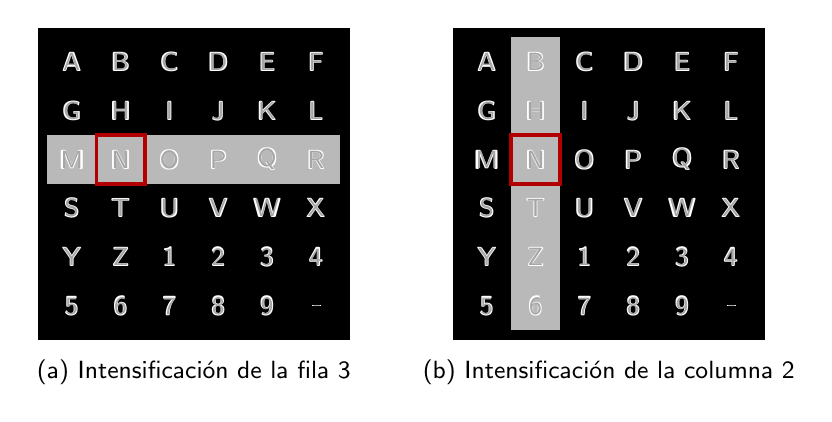
\begin{tikzpicture}[scale=0.62, every node/.style={font=\sffamily\small}]
  \def\letras{{"A","B","C","D","E","F","G","H","I","J","K","L","M","N","O","P","Q","R",
               "S","T","U","V","W","X","Y","Z","1","2","3","4","5","6","7","8","9","\_"}}
  % matriz izquierda: fila 3 intensificada
  \begin{scope}
    \fill[black] (-0.2,-0.2) rectangle (6.2,6.2);
    \fill[gray!55] (0,3) rectangle (6,4);
    \foreach \i in {0,...,35}{
      \pgfmathtruncatemacro{\f}{int(\i/6)}
      \pgfmathtruncatemacro{\c}{mod(\i,6)}
      \pgfmathsetmacro{\l}{\letras[\i]}
      \ifthenelse{\f=2}
        {\node[text=white, font=\sffamily\bfseries] at (\c+0.5,5.5-\f) {\l};}
        {\node[text=gray!70] at (\c+0.5,5.5-\f) {\l};}
    }
    \draw[red!70!black, very thick] (1,3) rectangle (2,4);
    \node[below, align=center] at (3,-0.4) {(a) Intensificación de la fila 3};
  \end{scope}
  % matriz derecha: columna 2 intensificada
  \begin{scope}[xshift=8.5cm]
    \fill[black] (-0.2,-0.2) rectangle (6.2,6.2);
    \fill[gray!55] (1,0) rectangle (2,6);
    \foreach \i in {0,...,35}{
      \pgfmathtruncatemacro{\f}{int(\i/6)}
      \pgfmathtruncatemacro{\c}{mod(\i,6)}
      \pgfmathsetmacro{\l}{\letras[\i]}
      \ifthenelse{\c=1}
        {\node[text=white, font=\sffamily\bfseries] at (\c+0.5,5.5-\f) {\l};}
        {\node[text=gray!70] at (\c+0.5,5.5-\f) {\l};}
    }
    \draw[red!70!black, very thick] (1,3) rectangle (2,4);
    \node[below, align=center] at (3,-0.4) {(b) Intensificación de la columna 2};
  \end{scope}
\end{tikzpicture}
\caption{Matriz de $6\times6$ caracteres del P300 Speller. Si el usuario atiende a la letra N
(recuadro), tanto la intensificación de la fila 3 como la de la columna 2 son eventos objetivo que
provocan una P300; las diez intensificaciones restantes son eventos no objetivo. Elaboración propia
con base en \cite{farwell1988}.}
\label{fig:matriz}
\end{figure}

El sistema original registraba el EEG únicamente en el electrodo Pz y, con cuatro participantes
sanos, alcanzó una exactitud cercana al 95\% con un tiempo promedio de 26 segundos por carácter,
equivalente a 2.3 caracteres o 12 bits por minuto \cite{farwell1988}. Aunque esta velocidad es muy
baja comparada con la escritura convencional, la arquitectura y el principio de operación de este
deletreador siguen siendo la base de la mayoría de los sistemas BCI basados en la P300
\cite{contreras2021}.

\subsection{Parámetros de estimulación}

El desempeño del P300 Speller depende en buena medida de los tiempos con que se presentan los
estímulos. La duración de la intensificación indica el tiempo durante el cual una fila o columna
permanece iluminada; el intervalo entre estímulos (ISI) corresponde al tiempo en que la matriz
permanece sin intensificar antes del siguiente evento; y la suma de ambos define el intervalo entre
inicios de estímulos (SOA). A una secuencia completa de las doce intensificaciones se le llama
repetición, y el número de repeticiones que se realizan antes de decidir el carácter determina el
compromiso entre velocidad y exactitud \cite{krusienski2008}. La Figura~\ref{fig:tiempos}
representa estos parámetros con los valores de la base de datos II de la tercera competencia BCI,
utilizada en este trabajo, en la que cada intensificación dura 100~ms seguida de 75~ms sin
estímulo, y cada carácter se deletrea con 15 repeticiones, es decir, con 180 intensificaciones
\cite{blankertz2006}.

\begin{figure}[htbp]
\centering
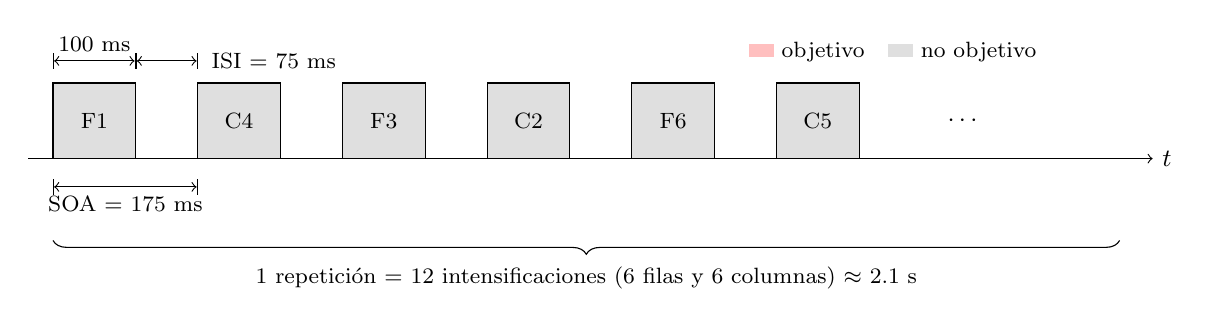
\begin{tikzpicture}[x=1.05cm, y=0.8cm, font=\small]
  % señal de estimulación
  \draw[->] (0,0) -- (13.6,0) node[right] {$t$};
  \foreach \k/\et/\obj in {0/F1/0,1/C4/0,2/F3/1,3/C2/1,4/F6/0,5/C5/0}{
    \pgfmathsetmacro{\xa}{\k*1.75+0.3}
    \pgfmathsetmacro{\xb}{\xa+1.0}
    \ifthenelse{\obj=1}
      {\fill[red!25] (\xa,0) rectangle (\xb,1.2);}
      {\fill[gray!25] (\xa,0) rectangle (\xb,1.2);}
    \draw (\xa,0) rectangle (\xb,1.2);
    \node at ({\xa+0.5},0.6) {\footnotesize \et};
  }
  \node at (11.3,0.6) {$\cdots$};
  % cotas
  \draw[|<->|] (0.3,1.55) -- node[above, font=\footnotesize] {100 ms} (1.3,1.55);
  \draw[|<->|] (1.3,1.55) -- (2.05,1.55); \node[font=\footnotesize, anchor=west] at (2.1,1.55) {ISI = 75 ms};
  \draw[|<->|] (0.3,-0.45) -- node[below, font=\footnotesize] {SOA = 175 ms} (2.05,-0.45);
  \draw[decorate, decoration={brace, amplitude=5pt, mirror}] (0.3,-1.3) -- node[below=6pt, font=\footnotesize, align=center] {1 repetición = 12 intensificaciones (6 filas y 6 columnas) $\approx$ 2.1 s} (13.2,-1.3);
  \node[font=\footnotesize, align=left, anchor=west] at (8.6,1.7) {\tikz\fill[red!25] (0,0) rectangle (0.3,0.2); objetivo\quad \tikz\fill[gray!25] (0,0) rectangle (0.3,0.2); no objetivo};
\end{tikzpicture}
\caption{Parámetros de estimulación del P300 Speller con los valores de la base de datos II de la
competencia BCI III (F = fila, C = columna). Elaboración propia con base en \cite{blankertz2006}.}
\label{fig:tiempos}
\end{figure}

\subsection{Épocas de EEG y decodificación del carácter}

Para clasificar la señal, el registro continuo se divide en segmentos que inician en el instante
de cada intensificación, llamados épocas. Siguiendo la notación de Mercado \cite{mercado2016},
retomada por Contreras \cite{contreras2021}, una sesión de registro puede expresarse como
$x_{i,ch}(n)$, donde $i$ es el número de registro, $ch$ el canal y $n=1,2,\dots,N$ las muestras;
una época se denota como $x^{k,y}_{i,ch}(n)$, donde $k\in\{a,u\}$ indica si se trata de una época
atendida, sincronizada con una fila o columna que contiene al carácter objetivo, o no atendida, y
$y\in\{f,c\}$ indica si la intensificación correspondió a una fila o a una columna.

Una vez que un clasificador asigna a cada época un puntaje $g(\cdot)$ que refleja la probabilidad
de que contenga una P300, el carácter se decide sumando los puntajes de cada fila y cada columna a
lo largo de las $J$ repeticiones y eligiendo aquellas con el valor más alto \cite{rakotomamonjy2008}:
\begin{equation}
\hat{f} = \arg\max_{f\in\{1,\dots,6\}} \sum_{j=1}^{J} g\!\left(x^{f}_{j}\right), \qquad
\hat{c} = \arg\max_{c\in\{1,\dots,6\}} \sum_{j=1}^{J} g\!\left(x^{c}_{j}\right),
\label{eq:decodificacion}
\end{equation}
de modo que el carácter seleccionado es el que se encuentra en la intersección de la fila
$\hat{f}$ y la columna $\hat{c}$. Con esta estrategia, el ganador de la competencia BCI III
alcanzó una exactitud del 96.5\% al utilizar las 15 repeticiones disponibles
\cite{rakotomamonjy2008}.

Cabe destacar que, por la propia estructura del paradigma, el conjunto de épocas está fuertemente
desbalanceado: en cada repetición solo dos de las doce intensificaciones son objetivo, lo que
produce una proporción de una época positiva por cada cinco negativas \cite{cecotti2011}. Si este
desbalance no se considera durante el entrenamiento, un clasificador puede alcanzar una exactitud
aparente cercana al 83\% simplemente prediciendo siempre la clase negativa, razón por la cual las
métricas de evaluación de la Sección~\ref{sec:metricas} deben elegirse con cuidado.

\subsection{Variantes del paradigma}

El paradigma de filas y columnas presenta algunos problemas conocidos. Los errores de adyacencia
ocurren cuando el sistema selecciona un carácter vecino al objetivo, debido a que las
intensificaciones de filas o columnas contiguas también atraen parcialmente la atención del
usuario, y el problema del doble destello aparece cuando la misma fila o columna objetivo se
intensifica dos veces seguidas, de forma que la segunda P300 se atenúa o se traslapa con la
primera \cite{townsend2010}. Para mitigarlos se han propuesto distintas variantes, resumidas en la
Tabla~\ref{tab:variantes}, entre las que destacan el paradigma de tablero de ajedrez de Townsend et
al., que intensifica grupos de caracteres no contiguos \cite{townsend2010}, y el uso de rostros
conocidos superpuestos a los caracteres, con el que Kaufmann et al. obtuvieron ERP de mayor
amplitud y redujeron el número de secuencias necesarias para una selección correcta
\cite{kaufmann2011}.

\begin{table}[htbp]
\centering
\caption{Variantes del paradigma de estimulación del P300 Speller}
\label{tab:variantes}
\small
\begin{tabularx}{\textwidth}{L{3.0cm}YY}
\toprule
\textbf{Variante} & \textbf{Descripción} & \textbf{Ventajas y desventajas} \\
\midrule
Filas y columnas \cite{farwell1988} & Se intensifica una fila o columna completa a la vez. & Solo 12 eventos por repetición; sufre errores de adyacencia y doble destello. \\
Carácter único \cite{guger2009} & Se intensifica un solo carácter a la vez. & P300 de mayor amplitud por ser más infrecuente, pero requiere 36 eventos por repetición y resultó menos exacto en \cite{guger2009}. \\
Tablero de ajedrez \cite{townsend2010} & Se intensifican grupos de caracteres que no comparten fila ni columna. & Reduce errores de adyacencia y doble destello; mayor complejidad en el diseño de los grupos. \\
Estímulos con rostros \cite{kaufmann2011} & Se superpone la imagen de un rostro conocido sobre los caracteres. & ERP de mayor amplitud y menos repeticiones; requiere estímulos visuales más elaborados. \\
\bottomrule
\end{tabularx}
\par\smallskip{\footnotesize Elaboración propia.}
\end{table}

\subsection{Bases de datos públicas}

Gran parte de la investigación sobre detección de la P300 se apoya en bases de datos públicas, lo
que permite comparar métodos bajo las mismas condiciones sin tener que adquirir señales propias.
Las más utilizadas provienen de la segunda y tercera competencias internacionales de BCI, ambas
registradas con 64 canales a 240~Hz con el paradigma de filas y columnas
\cite{blankertz2004,blankertz2006}, mientras que la base de datos de la Escuela Politécnica Federal
de Lausana (EPFL) incluye registros de personas con discapacidad motora con un paradigma de seis
imágenes \cite{hoffmann2008}. La Tabla~\ref{tab:datasets} resume sus características; en el
presente trabajo se emplea la base de datos II de la competencia BCI III, que contiene registros de
dos sujetos con 85 caracteres de entrenamiento y 100 de prueba cada uno.

\begin{table}[htbp]
\centering
\caption{Bases de datos públicas del paradigma P300}
\label{tab:datasets}
\small
\begin{tabularx}{\textwidth}{L{3.3cm}L{1.4cm}L{1.4cm}L{1.4cm}Y}
\toprule
\textbf{Base de datos} & \textbf{Sujetos} & \textbf{Canales} & \textbf{Frec. (Hz)} & \textbf{Paradigma} \\
\midrule
BCI Competition II, conjunto IIb \cite{blankertz2004} & 1 & 64 & 240 & Matriz $6\times6$, filas y columnas, 15 repeticiones. \\
BCI Competition III, conjunto II \cite{blankertz2006} & 2 & 64 & 240 & Matriz $6\times6$, filas y columnas, 15 repeticiones; 85 caracteres de entrenamiento y 100 de prueba por sujeto. \\
EPFL \cite{hoffmann2008} & 8 & 32 & 2048 & Seis imágenes intensificadas de una en una; incluye sujetos con discapacidad motora. \\
\bottomrule
\end{tabularx}
\par\smallskip{\footnotesize Elaboración propia.}
\end{table}

% ---------------------------------------------------------------------
% 2.7 Procesamiento digital de señales biomédicas
% ---------------------------------------------------------------------
\section[PROCESAMIENTO DIGITAL DE SEÑALES BIOMÉDICAS]{Procesamiento Digital de Señales
Biomédicas}
\label{sec:pds}

El preprocesamiento de las señales EEG constituye una etapa determinante para el desempeño de
los modelos de clasificación, dado que estas señales presentan una relación señal-ruido baja y
son susceptibles a artefactos de origen fisiológico y ambiental. Para atender esta problemática
se emplean técnicas de filtrado pasa banda, orientadas a delimitar el rango de frecuencias
asociado a la componente P300, así como la segmentación de la señal continua en ventanas
temporales alrededor de cada estímulo y la normalización de las mismas, cuyos fundamentos se
describen a lo largo de esta sección.

\subsection{Muestreo y teorema de Nyquist}

Las señales de origen fisiológico son de naturaleza analógica, es decir, están definidas en todo
instante de tiempo y su amplitud puede tomar cualquier valor dentro de su rango dinámico; para
procesarlas en una computadora es necesario muestrearlas a intervalos regulares
$T_s = 1/f_s$, obteniendo la secuencia discreta $x(n) = x_a(nT_s)$ \cite{proakis2007}. El teorema
de muestreo establece que una señal cuyo contenido en frecuencia está limitado a $f_{\max}$ puede
reconstruirse sin pérdida a partir de sus muestras siempre que
\begin{equation}
f_s \geq 2 f_{\max},
\label{eq:nyquist}
\end{equation}
y si esta condición no se cumple, las componentes de frecuencia superiores a $f_s/2$, conocida
como frecuencia de Nyquist, se reflejan sobre las frecuencias bajas en un fenómeno llamado
\textit{aliasing} \cite{oppenheim2010}. La base de datos utilizada en este trabajo fue muestreada a
240~Hz, por lo que su frecuencia de Nyquist de 120~Hz está muy por encima de la banda de interés
de la P300, que se concentra por debajo de 20~Hz.

\subsection{Transformada de Fourier y densidad espectral de potencia}

La transformada discreta de Fourier (DFT) permite representar una secuencia de $N$ muestras como
una suma de componentes sinusoidales, y se define como
\begin{equation}
X(k) = \sum_{n=0}^{N-1} x(n)\, e^{-j 2\pi k n / N}, \qquad k = 0, 1, \dots, N-1,
\label{eq:dft}
\end{equation}
donde cada coeficiente $X(k)$ corresponde a la frecuencia $f_k = k f_s / N$; su cálculo directo
requiere del orden de $N^2$ operaciones, mientras que el algoritmo de la transformada rápida de
Fourier (FFT) lo reduce a $N\log_2 N$ \cite{proakis2007}. A partir de ella se estima la densidad
espectral de potencia (PSD), que describe cómo se distribuye la potencia de la señal en función
de la frecuencia. En el caso del EEG suele emplearse el método de Welch, que divide la señal en
segmentos traslapados, calcula el periodograma de cada uno y los promedia, reduciendo así la
varianza de la estimación a costa de una menor resolución en frecuencia \cite{oppenheim2010}.
Contreras utilizó este análisis para identificar que la información útil para detectar la P300 en
sus registros se encontraba entre 1 y 25~Hz \cite{contreras2021}; la Figura~\ref{fig:psd} muestra
una PSD típica en la que se distinguen el pico del ritmo alfa y la interferencia de la red
eléctrica.

\begin{figure}[htbp]
\centering

\includegraphics[width=0.8\textwidth]{02-marco-referencial/psd_welch.pdf}
\caption{Densidad espectral de potencia estimada con el método de Welch para una señal de EEG
sintética. Elaboración propia.}
\label{fig:psd}
\end{figure}

\subsection{Convolución y sistemas lineales}

Un sistema lineal e invariante en el tiempo queda completamente descrito por su respuesta al
impulso $h(n)$, y su salida ante cualquier entrada $x(n)$ se obtiene mediante la operación de
convolución \cite{proakis2007}:
\begin{equation}
y(n) = (x * h)(n) = \sum_{k=-\infty}^{\infty} x(k)\, h(n-k).
\label{eq:convolucion}
\end{equation}
Esta operación es la base de los filtros digitales que se describen a continuación y, como se
verá en la Sección~\ref{sec:cnn}, también de las capas de las redes neuronales convolucionales,
en las que los coeficientes de $h(n)$ ya no se diseñan manualmente sino que se aprenden a partir
de los datos \cite{goodfellow2016}.

\subsection{Filtros digitales}

Los filtros digitales se clasifican en dos grandes familias según la duración de su respuesta al
impulso. Los filtros de respuesta finita al impulso (FIR) calculan la salida únicamente a partir de
las muestras de entrada, son siempre estables y pueden diseñarse con fase lineal, mientras que los
de respuesta infinita al impulso (IIR) utilizan además salidas anteriores, lo que les permite
lograr una transición más abrupta con un orden mucho menor, aunque con una respuesta de fase no
lineal \cite{proakis2007,oppenheim2010}. Entre los filtros IIR, el de Butterworth es uno de los más
utilizados en EEG porque su respuesta en magnitud es máximamente plana en la banda de paso
\cite{oppenheim2010}. De acuerdo con la banda que dejan pasar, los filtros pueden ser pasa bajas,
pasa altas, pasa banda o rechaza banda; un caso particular de estos últimos es el filtro
\textit{notch}, diseñado para eliminar una sola frecuencia como la de la red eléctrica. La
Tabla~\ref{tab:filtros} resume sus características y la Figura~\ref{fig:filtros} muestra la
respuesta en frecuencia de un filtro pasa banda entre 0.1 y 20~Hz, como el aplicado en el trabajo
preliminar, y de un filtro \textit{notch} en 60~Hz.

\begin{table}[htbp]
\centering
\caption{Comparación de filtros digitales FIR e IIR}
\label{tab:filtros}
\small
\begin{tabularx}{\textwidth}{L{3.3cm}YY}
\toprule
\textbf{Característica} & \textbf{FIR} & \textbf{IIR (p.\,ej. Butterworth)} \\
\midrule
Ecuación en diferencias & $y(n)=\sum_{k=0}^{M} b_k\,x(n-k)$ & $y(n)=\sum_{k=0}^{M} b_k\,x(n-k)-\sum_{k=1}^{N} a_k\,y(n-k)$ \\
Estabilidad & Siempre estable. & Depende de la ubicación de los polos. \\
Fase & Puede ser lineal (retardo constante). & No lineal; se compensa con filtrado hacia adelante y hacia atrás. \\
Orden necesario & Alto para transiciones abruptas. & Bajo para la misma selectividad. \\
Costo computacional & Mayor. & Menor. \\
\bottomrule
\end{tabularx}
\par\smallskip{\footnotesize Elaboración propia con información de \cite{proakis2007,oppenheim2010}.}
\end{table}

\begin{figure}[htbp]
\centering

\includegraphics[width=\textwidth]{02-marco-referencial/respuesta_filtros.pdf}
\caption{Respuesta en magnitud de (a) un filtro pasa banda Butterworth de cuarto orden entre 0.1 y
20~Hz y (b) un filtro \textit{notch} en 60~Hz, para $f_s = 240$~Hz. Elaboración propia.}
\label{fig:filtros}
\end{figure}

\subsection{Filtrado de fase cero y remuestreo}

La fase no lineal de los filtros IIR provoca que distintas frecuencias se retrasen de forma
diferente, lo que puede desplazar el pico de un ERP y alterar la latencia medida de la P300
\cite{luck2014}. Cuando el procesamiento se realiza fuera de línea, este efecto se elimina
aplicando el filtro dos veces, una en sentido directo y otra en sentido inverso, técnica conocida
como filtrado de fase cero, que duplica la atenuación efectiva del filtro sin introducir retardo
\cite{oppenheim2010}. Por otra parte, el remuestreo permite reducir la frecuencia de muestreo una
vez que la señal ya fue filtrada; en la decimación por un factor $M$ se conserva una de cada $M$
muestras, siempre que antes se haya aplicado un filtro antialiasing que elimine el contenido por
encima de la nueva frecuencia de Nyquist \cite{proakis2007}. En el trabajo preliminar se redujo la
frecuencia de 240~Hz a 120~Hz, lo que disminuye a la mitad el tamaño de cada época sin perder
información en la banda de 0.1 a 20~Hz.

\subsection{Referencia y corrección de línea base}

Además del filtrado en frecuencia, es común modificar la referencia de los canales después del
registro. La referencia promedio común resta a cada canal $x_{ch}(n)$ el promedio de los $C$
canales en cada instante,
\begin{equation}
x^{\text{CAR}}_{ch}(n) = x_{ch}(n) - \frac{1}{C}\sum_{c=1}^{C} x_{c}(n),
\label{eq:car}
\end{equation}
con lo que se atenúan las componentes comunes a todos los electrodos, como las derivadas de la
propia referencia \cite{luck2014}. De forma complementaria, la corrección de línea base resta a
cada época el valor promedio de un intervalo previo al estímulo, típicamente de 100 a 200~ms, para
que las amplitudes de los componentes del ERP se midan respecto a un nivel común \cite{luck2014}.

\subsection{Segmentación en épocas}

La segmentación consiste en dividir la señal continua en ventanas sincronizadas con cada estímulo,
que constituyen las muestras de entrada al clasificador. La longitud de la ventana debe ser
suficiente para contener la P300 completa; Contreras empleó ventanas de 1005~ms a partir del
estímulo \cite{contreras2021}, mientras que en el trabajo preliminar se utilizaron ventanas de 78
muestras, equivalentes a unos 650~ms a 120~Hz. Dado que el intervalo entre inicios de estímulos es
de solo 175~ms, las épocas de intensificaciones consecutivas se traslapan, como se observa en la
Figura~\ref{fig:epocas}, de modo que una época no objetivo puede contener parte de la P300
provocada por una intensificación objetivo cercana.

\begin{figure}[htbp]
\centering

\includegraphics[width=\textwidth]{02-marco-referencial/segmentacion_epocas.pdf}
\caption{Segmentación de la señal continua en épocas de 0 a 650~ms a partir de cada
intensificación. Señal sintética, elaboración propia.}
\label{fig:epocas}
\end{figure}

\subsection{Normalización}

Las amplitudes del EEG varían entre canales, sesiones y sujetos, por lo que antes de entrenar un
modelo se acostumbra normalizar los datos. La normalización \textit{z-score} transforma cada canal
para que tenga media cero y desviación estándar unitaria, mientras que la normalización
\textit{min-max}, utilizada por Contreras \cite{contreras2021}, escala los valores al intervalo
$[0,1]$:
\begin{equation}
z(n) = \frac{x(n)-\mu}{\sigma}, \qquad
x'(n) = \frac{x(n)-\min(x)}{\max(x)-\min(x)}.
\label{eq:normalizacion}
\end{equation}
La primera es menos sensible a valores atípicos, lo cual resulta conveniente en presencia de
artefactos de gran amplitud, y fue la empleada de manera independiente por canal en el trabajo
preliminar para evitar que los electrodos con mayor amplitud dominen el aprendizaje de la red.

\subsection{Remoción de artefactos}

Cuando los artefactos se traslapan en frecuencia con la señal de interés, como ocurre con los
parpadeos y la banda de la P300, el filtrado no basta para eliminarlos. La estrategia más simple
consiste en descartar las épocas cuya amplitud supere un umbral, aunque esto reduce la cantidad de
datos disponibles; como alternativa, el análisis de componentes independientes (ICA) separa la
señal multicanal en fuentes estadísticamente independientes, de modo que las asociadas a
movimientos oculares o musculares pueden identificarse y eliminarse antes de reconstruir el EEG
\cite{jung2000}. Esta técnica se popularizó gracias a herramientas como EEGLAB, que la integran
junto con otras rutinas de análisis de ensayos individuales \cite{delorme2004}.

\subsection{Filtrado espacial}

Finalmente, además de filtrar cada canal en el tiempo, es posible combinar los canales mediante un
filtro espacial que realce la señal de interés. El algoritmo xDAWN, propuesto por Rivet et al.,
estima los filtros espaciales que maximizan la relación entre la señal evocada y la señal más
ruido, y ha mostrado mejorar la detección de la P300 aun con un número reducido de canales
\cite{rivet2009}. Este tipo de filtrado es, en cierto sentido, lo que las capas convolucionales
espaciales de redes como EEGNet aprenden de manera automática a partir de los datos
\cite{lawhern2018}.

% ---------------------------------------------------------------------
% 2.8 Inteligencia artificial y aprendizaje automático
% ---------------------------------------------------------------------
\section[INTELIGENCIA ARTIFICIAL Y APRENDIZAJE AUTOMÁTICO]{Inteligencia Artificial y aprendizaje
automático}

La inteligencia artificial (IA) es la rama de las ciencias de la computación que estudia el
diseño de agentes capaces de percibir su entorno y actuar de manera que maximicen la probabilidad
de alcanzar sus objetivos, automatizando actividades que se asocian con el pensamiento humano, como
la resolución de problemas y el aprendizaje \cite{russell2010}. No existe un método universal para
todas las áreas de aplicación de la IA, y dentro de la gran variedad de enfoques disponibles el
aprendizaje automático se ha convertido en una de sus ramas más importantes \cite{ertel2017}. A su
vez, el aprendizaje profundo es un subconjunto del aprendizaje automático basado en redes
neuronales con múltiples capas de procesamiento, relación que se ilustra en la
Figura~\ref{fig:ia}.

\begin{figure}[htbp]
\centering
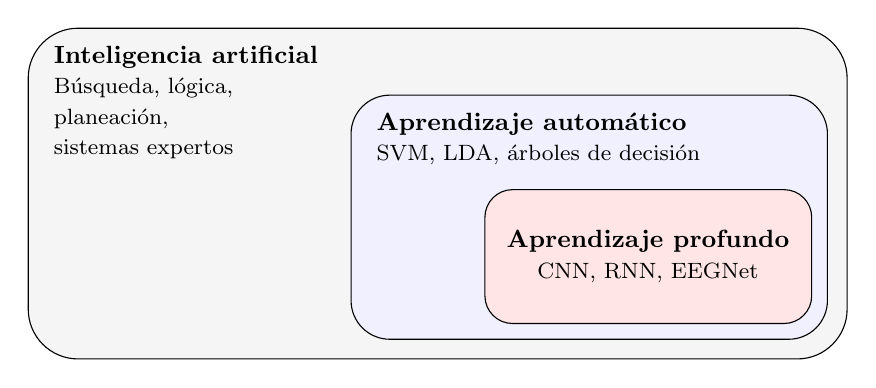
\begin{tikzpicture}[font=\small]
  \draw[fill=gray!8, rounded corners=18pt] (-5.2,-2.1) rectangle (5.2,2.1);
  \node[anchor=north west, align=left] at (-5.0,2.0) {\textbf{Inteligencia artificial}\\ \footnotesize Búsqueda, lógica,\\ \footnotesize planeación,\\ \footnotesize sistemas expertos};
  \draw[fill=blue!6, rounded corners=14pt] (-1.1,-1.85) rectangle (4.95,1.25);
  \node[anchor=north west, align=left] at (-0.9,1.15) {\textbf{Aprendizaje automático}\\ \footnotesize SVM, LDA, árboles de decisión};
  \draw[fill=red!10, rounded corners=10pt] (0.6,-1.65) rectangle (4.75,0.05);
  \node[align=center] at (2.67,-0.8) {\textbf{Aprendizaje profundo}\\ \footnotesize CNN, RNN, EEGNet};
\end{tikzpicture}
\caption{Relación entre la inteligencia artificial, el aprendizaje automático y el aprendizaje
profundo. Elaboración propia con base en \cite{goodfellow2016}.}
\label{fig:ia}
\end{figure}

\subsection{Aprendizaje automático}

En 1959, Arthur Samuel describió el aprendizaje automático como el campo de estudio que da a las
computadoras la capacidad de aprender sin ser programadas de forma explícita, a partir de su
experiencia con un programa que aprendía a jugar damas mejor que su propio creador
\cite{samuel1959}. En términos más formales, se trata de un conjunto de métodos que construyen
modelos a partir de los datos mediante el descubrimiento de patrones estadísticamente
significativos, para después aplicarlos a datos nuevos de la misma naturaleza \cite{bishop2006}.
Dependiendo de la información disponible durante el entrenamiento, se distinguen los tres tipos de
aprendizaje que se presentan en la Tabla~\ref{tab:tipos-ml}; la detección de la P300 corresponde a
un problema de clasificación binaria supervisada, pues cada época está etiquetada como objetivo o
no objetivo.

\begin{table}[htbp]
\centering
\caption{Tipos de aprendizaje automático}
\label{tab:tipos-ml}
\small
\begin{tabularx}{\textwidth}{L{2.6cm}YY}
\toprule
\textbf{Tipo} & \textbf{Descripción} & \textbf{Ejemplos de tareas} \\
\midrule
Supervisado & El modelo aprende una función que relaciona entradas con etiquetas conocidas, ajustando sus parámetros según el error entre la salida y la etiqueta. & Clasificación de épocas P300 / no P300; regresión. \\
No supervisado & El modelo busca estructura en datos sin etiquetas, agrupándolos o reduciendo su dimensión. & Agrupamiento, ICA, análisis de componentes principales. \\
Por refuerzo & Un agente aprende por prueba y error a partir de recompensas asociadas a sus acciones. & Control, juegos, adaptación en línea de una BCI. \\
\bottomrule
\end{tabularx}
\par\smallskip{\footnotesize Elaboración propia con información de \cite{bishop2006,russell2010}.}
\end{table}

\subsection{Clasificadores clásicos para la detección de la P300}

Antes del auge del aprendizaje profundo, la detección de la P300 se realizaba extrayendo
características de manera manual, generalmente las amplitudes de la señal submuestreada en cada
canal, y clasificándolas con modelos lineales. Krusienski et al. compararon cinco técnicas de
clasificación para el P300 Speller y encontraron que el análisis discriminante lineal por pasos
(SWLDA) y el discriminante lineal de Fisher ofrecían el mejor desempeño global
\cite{krusienski2006}, mientras que Rakotomamonjy y Guigue ganaron la competencia BCI III con un
conjunto de máquinas de soporte vectorial (SVM) lineales entrenadas sobre distintas particiones de
los datos \cite{rakotomamonjy2008}. En el ámbito de la ESCOM, Santos, Romero y Fernández utilizaron
el discriminante lineal de Fisher con promediado sincronizado para controlar un brazo robótico
virtual, alcanzando una precisión de 90.01\% con 20 sujetos \cite{santos2017}. La
Tabla~\ref{tab:clasicos} resume estos métodos.

\begin{table}[htbp]
\centering
\caption{Clasificadores clásicos utilizados en la detección de la P300}
\label{tab:clasicos}
\small
\begin{tabularx}{\textwidth}{L{2.4cm}YYY}
\toprule
\textbf{Clasificador} & \textbf{Descripción} & \textbf{Ventajas} & \textbf{Desventajas} \\
\midrule
LDA / Fisher \cite{krusienski2006,santos2017} & Proyecta los datos sobre la dirección que maximiza la separación entre las medias de las clases respecto a su dispersión. & Simple, rápido y con pocos parámetros; buen desempeño en P300. & Supone clases gaussianas con igual covarianza; sensible con muchas características. \\
SWLDA \cite{krusienski2006} & LDA con selección de características por pasos (se agregan o eliminan según su significancia estadística). & Reduce la dimensión y el sobreajuste; de los mejores en la comparación de \cite{krusienski2006}. & Selección costosa con muchos canales. \\
SVM lineal \cite{rakotomamonjy2008} & Busca el hiperplano que maximiza el margen entre clases. & Robusta en alta dimensión; ganó la competencia BCI III. & Requiere ajustar el parámetro de regularización; entrenamiento más lento. \\
\bottomrule
\end{tabularx}
\par\smallskip{\footnotesize Elaboración propia.}
\end{table}

\subsection{Sobreajuste y generalización}

El objetivo de un modelo de aprendizaje automático no es reproducir los datos con los que fue
entrenado sino desempeñarse correctamente con datos que nunca ha visto, capacidad conocida como
generalización \cite{goodfellow2016}. Cuando un modelo es demasiado complejo para la cantidad de
datos disponibles, o cuando se entrena durante demasiadas iteraciones, comienza a memorizar el
ruido particular del conjunto de entrenamiento: el error de entrenamiento sigue disminuyendo
mientras que el error de validación deja de bajar y empieza a crecer, fenómeno conocido como
sobreajuste y que se ilustra en la Figura~\ref{fig:sobreajuste} \cite{goodfellow2016,bishop2006}.
En el caso del EEG este riesgo es particularmente alto, pues las bases de datos suelen contener
pocos sujetos y un número limitado de épocas objetivo.

\begin{figure}[htbp]
\centering

\includegraphics[width=0.68\textwidth]{02-marco-referencial/sobreajuste.pdf}
\caption{Curvas de pérdida de entrenamiento y validación: a partir de cierto punto el modelo
comienza a sobreajustarse. Elaboración propia.}
\label{fig:sobreajuste}
\end{figure}

\subsection{Esquemas de validación}

Para estimar la capacidad de generalización, los datos se dividen en un conjunto de
entrenamiento, uno de validación, que se usa para ajustar hiperparámetros y decidir cuándo
detener el entrenamiento, y uno de prueba, que solo se utiliza al final \cite{goodfellow2016}. La
validación cruzada de $k$ particiones repite este proceso $k$ veces rotando el subconjunto de
validación, lo que ofrece una estimación más estable cuando hay pocos datos \cite{bishop2006}. En
las BCI, además, es importante distinguir entre la evaluación intrasujeto, en la que el modelo se
entrena y se prueba con datos de la misma persona, y la evaluación intersujeto, en la que se prueba
con una persona que no participó en el entrenamiento, ya sea mediante el esquema de dejar un sujeto
fuera o entrenando con sujetos distintos \cite{alvarado2021}. Contreras evaluó ambos escenarios y
obtuvo valores promedio de AUC cercanos a 0.82 en la evaluación intrasujeto y de 0.70 en la
intersujeto al considerar filas y columnas en conjunto \cite{contreras2021}.

% ---------------------------------------------------------------------
% 2.9 Redes neuronales artificiales y aprendizaje profundo
% ---------------------------------------------------------------------
\section[REDES NEURONALES ARTIFICIALES Y APRENDIZAJE PROFUNDO]{Redes neuronales artificiales y
aprendizaje profundo}

\subsection{La neurona artificial}

Las redes neuronales artificiales son modelos inspirados en el sistema nervioso, en los que las
unidades de cómputo, llamadas neuronas, se conectan entre sí mediante pesos que cumplen un papel
análogo al de la fuerza de las conexiones sinápticas en los organismos biológicos
\cite{aggarwal2018}. Cada neurona recibe un vector de entradas $\mathbf{x} = (x_1, \dots, x_n)$,
las multiplica por sus pesos $w_i$, suma el resultado junto con un sesgo $b$ y aplica una función
de activación $\varphi$ no lineal \cite{delbrio2002}:
\begin{equation}
y = \varphi\!\left(\sum_{i=1}^{n} w_i x_i + b\right) = \varphi\!\left(\mathbf{w}^{\top}\mathbf{x} + b\right).
\label{eq:neurona}
\end{equation}
La Figura~\ref{fig:neurona} muestra la correspondencia entre este modelo y la neurona biológica
descrita en la Sección~\ref{sec:neuro}: las entradas desempeñan el papel de las dendritas, la suma ponderada
el del soma y la salida el del axón. Al organizar muchas de estas unidades en capas, de manera que
la salida de una capa sea la entrada de la siguiente, se obtiene el perceptrón multicapa, en el que
las capas intermedias se denominan ocultas; al número de capas se le conoce como profundidad de la
red, y de ahí proviene el término aprendizaje profundo \cite{goodfellow2016}.

\begin{figure}[htbp]
\centering
\begin{tikzpicture}[
  ent/.style={circle, draw, minimum size=0.75cm, font=\small},
  flecha/.style={-{Stealth[length=2mm]}, thick}]
  \node[ent] (x1) at (0,1.6) {$x_1$};
  \node[ent] (x2) at (0,0.5) {$x_2$};
  \node at (0,-0.35) {$\vdots$};
  \node[ent] (xn) at (0,-1.2) {$x_n$};
  \node[ent] (b) at (1.9,2.1) {$1$};
  \node[circle, draw, thick, minimum size=1.2cm, fill=gray!10] (sum) at (3.6,0.3) {$\Sigma$};
  \node[rectangle, draw, thick, minimum size=1.0cm, fill=red!8] (act) at (5.6,0.3) {$\varphi(\cdot)$};
  \node (y) at (7.4,0.3) {$y$};
  \draw[flecha] (x1) -- node[above, font=\footnotesize, sloped] {$w_1$} (sum);
  \draw[flecha] (x2) -- node[above, font=\footnotesize, sloped] {$w_2$} (sum);
  \draw[flecha] (xn) -- node[below, font=\footnotesize, sloped] {$w_n$} (sum);
  \draw[flecha] (b) -- node[above right, font=\footnotesize] {$b$} (sum);
  \draw[flecha] (sum) -- node[above, font=\footnotesize] {$z$} (act);
  \draw[flecha] (act) -- (y);
  \node[font=\footnotesize, align=center, text=gray] at (0,-2.2) {Entradas\\(dendritas)};
  \node[font=\footnotesize, align=center, text=gray] at (3.6,-1.25) {Suma ponderada\\(soma)};
  \node[font=\footnotesize, align=center, text=gray] at (5.6,-1.25) {Activación};
  \node[font=\footnotesize, align=center, text=gray] at (7.4,-0.5) {Salida\\(axón)};
\end{tikzpicture}
\caption{Modelo de la neurona artificial y su analogía con la neurona biológica. Elaboración
propia con base en \cite{aggarwal2018}.}
\label{fig:neurona}
\end{figure}

\subsection{Funciones de activación}

Sin la función de activación, una red de cualquier profundidad sería equivalente a una sola
transformación lineal, por lo que esta es la que permite a la red representar relaciones no
lineales \cite{goodfellow2016}. Las funciones sigmoide y tangente hiperbólica fueron las más
utilizadas en las primeras redes, y siguen empleándose en la capa de salida de los clasificadores
binarios y en arquitecturas para P300 como la de Cecotti y Gräser o SepConv1D
\cite{cecotti2011,alvarado2021}; sin embargo, ambas se saturan para valores grandes de su
entrada, lo que hace que sus gradientes tiendan a cero y dificulta el entrenamiento de redes
profundas. La función ReLU resolvió en gran medida este problema y hoy es la opción por defecto en
las capas ocultas \cite{goodfellow2016}, mientras que la ELU, utilizada en EEGNet, permite valores
negativos suaves que acercan la media de las activaciones a cero \cite{lawhern2018}. La
Tabla~\ref{tab:activaciones} presenta su definición y la Figura~\ref{fig:activaciones} su forma.

\begin{table}[htbp]
\centering
\caption{Funciones de activación más utilizadas}
\label{tab:activaciones}
\small
\begin{tabularx}{\textwidth}{L{2.6cm}L{4.3cm}L{1.6cm}Y}
\toprule
\textbf{Función} & \textbf{Definición} & \textbf{Rango} & \textbf{Uso típico} \\
\midrule
Sigmoide & $\sigma(z) = \dfrac{1}{1+e^{-z}}$ & $(0,1)$ & Salida de clasificación binaria (probabilidad de P300). \\[8pt]
Tangente hiperbólica & $\tanh(z) = \dfrac{e^{z}-e^{-z}}{e^{z}+e^{-z}}$ & $(-1,1)$ & Capas ocultas en \cite{cecotti2011,alvarado2021}; redes recurrentes. \\[8pt]
ReLU & $\max(0,z)$ & $[0,\infty)$ & Capas ocultas de redes profundas. \\[4pt]
ELU & $z$ si $z>0$; $\alpha(e^{z}-1)$ si $z\le0$ & $(-\alpha,\infty)$ & Capas ocultas de EEGNet \cite{lawhern2018}. \\[4pt]
Softmax & $\dfrac{e^{z_k}}{\sum_{j} e^{z_j}}$ & $(0,1)$, suma 1 & Salida de clasificación multiclase. \\
\bottomrule
\end{tabularx}
\par\smallskip{\footnotesize Elaboración propia con información de \cite{goodfellow2016,aggarwal2018}.}
\end{table}

\begin{figure}[htbp]
\centering

\includegraphics[width=\textwidth]{02-marco-referencial/funciones_activacion.pdf}
\caption{Gráfica de las funciones de activación sigmoide, tangente hiperbólica, ReLU y ELU.
Elaboración propia.}
\label{fig:activaciones}
\end{figure}

\subsection{Función de pérdida}

El entrenamiento de una red consiste en ajustar sus pesos para minimizar una función de pérdida
que mide la diferencia entre la salida de la red y la etiqueta esperada. Para la clasificación
binaria, con etiquetas $y_i\in\{0,1\}$ y salidas $\hat{y}_i\in(0,1)$, se utiliza la entropía
cruzada binaria \cite{goodfellow2016}:
\begin{equation}
\mathcal{L}_{\text{BCE}} = -\frac{1}{M}\sum_{i=1}^{M}\Big[\,y_i\log\hat{y}_i + (1-y_i)\log(1-\hat{y}_i)\Big].
\label{eq:bce}
\end{equation}
Debido al desbalance de las épocas del P300 Speller, en el que por cada época positiva hay cinco
negativas, es común ponderar el primer término con un factor $\alpha>1$ para que los errores sobre
la clase minoritaria tengan mayor peso, o bien emplear la pérdida focal, que multiplica cada
término por $(1-p_t)^{\gamma}$, donde $p_t$ es la probabilidad asignada a la clase correcta, para
reducir la contribución de los ejemplos que el modelo ya clasifica con facilidad \cite{lin2017}.

\subsection{Descenso de gradiente y retropropagación}

Para minimizar la pérdida se utiliza el método de descenso de gradiente, que actualiza los pesos
en la dirección opuesta al gradiente de la función de pérdida,
\begin{equation}
\mathbf{w}^{(t+1)} = \mathbf{w}^{(t)} - \eta\, \nabla_{\mathbf{w}}\mathcal{L}\big(\mathbf{w}^{(t)}\big),
\label{eq:gradiente}
\end{equation}
donde $\eta$ es la tasa de aprendizaje; si es muy pequeña el entrenamiento resulta lento, y si es
muy grande los pesos oscilan alrededor del mínimo sin alcanzarlo \cite{goodfellow2016}. El cálculo
eficiente de este gradiente en redes de varias capas se realiza mediante el algoritmo de
retropropagación, popularizado por Rumelhart, Hinton y Williams, que propaga el error desde la capa
de salida hacia las capas anteriores aplicando la regla de la cadena \cite{rumelhart1986}. En la
práctica el gradiente se estima sobre pequeños subconjuntos de datos llamados lotes, y en lugar de
una tasa fija se usan optimizadores adaptativos como Adam, que ajusta la tasa de aprendizaje de
cada parámetro a partir de estimaciones del primer y segundo momento de sus gradientes
\cite{kingma2015}, y que fue el utilizado en la comparación de arquitecturas para P300 de
Alvarado-González et al. \cite{alvarado2021}.

\subsection{Regularización}

Dado que las redes profundas tienen una gran cantidad de parámetros y los conjuntos de datos de EEG
son relativamente pequeños, es indispensable emplear técnicas de regularización para evitar el
sobreajuste. Entre las más utilizadas se encuentran el \textit{dropout}, que desactiva
aleatoriamente una fracción de las neuronas en cada iteración de entrenamiento
\cite{srivastava2014}, la normalización por lotes, que normaliza las activaciones de cada capa y
estabiliza el entrenamiento \cite{ioffe2015}, y la parada temprana, que detiene el entrenamiento
cuando la pérdida de validación deja de mejorar \cite{goodfellow2016}. A estas se suma la elección
de una inicialización adecuada de los pesos, como la propuesta por Glorot y Bengio, que mantiene la
varianza de las activaciones similar entre capas \cite{glorot2010}. La Tabla~\ref{tab:regularizacion}
resume estas técnicas junto con su uso en arquitecturas para la detección de la P300.

\begin{table}[htbp]
\centering
\caption{Técnicas de regularización y estabilización del entrenamiento}
\label{tab:regularizacion}
\small
\begin{tabularx}{\textwidth}{L{3.2cm}YY}
\toprule
\textbf{Técnica} & \textbf{Funcionamiento} & \textbf{Uso en P300} \\
\midrule
\textit{Dropout} \cite{srivastava2014} & Anula aleatoriamente una fracción $p$ de las activaciones durante el entrenamiento. & EEGNet y BN3 \cite{lawhern2018,liu2018}. \\
Normalización por lotes \cite{ioffe2015} & Normaliza la media y varianza de las activaciones de cada lote y las reescala con parámetros aprendidos. & BN3, EEGNet \cite{liu2018,lawhern2018}. \\
Regularización $L_2$ & Agrega a la pérdida un término proporcional a $\lVert\mathbf{w}\rVert^2$. & Modelos lineales y redes pequeñas. \\
Parada temprana & Detiene el entrenamiento cuando la pérdida de validación deja de mejorar durante cierto número de épocas. & 50 épocas de paciencia en \cite{alvarado2021}. \\
Inicialización de Glorot \cite{glorot2010} & Inicializa los pesos con una varianza dependiente del número de entradas y salidas de la capa. & Mayoría de las arquitecturas evaluadas en \cite{alvarado2021}. \\
\bottomrule
\end{tabularx}
\par\smallskip{\footnotesize Elaboración propia.}
\end{table}

\subsection{Aprendizaje profundo aplicado al EEG}

El aprendizaje profundo permite que los modelos aprendan representaciones de los datos con
múltiples niveles de abstracción directamente a partir de la señal, sin depender de
características diseñadas a mano \cite{lecun2015}. De acuerdo con Craik et al., un conjunto de
datos de EEG consiste, en su nivel más básico, en una matriz de dos dimensiones, canales por tiempo,
cuya estructura lo hace adecuado para este tipo de técnicas; en su revisión de 90 estudios
encontraron que las redes convolucionales, las recurrentes y las redes de creencia profunda
superaban en precisión a los autocodificadores apilados y a los perceptrones multicapa, y que para
las tareas de ERP se habían utilizado principalmente redes convolucionales, redes de creencia
profunda y autocodificadores \cite{craik2019}. Por su parte, la revisión sistemática de Roy et al.
señala que alrededor del 40\% de los estudios de aprendizaje profundo en EEG emplean redes
convolucionales \cite{roy2019}, mientras que Lotte et al. advierten que, en el momento de su revisión, las redes
profundas aún no mostraban una mejora contundente sobre los mejores métodos clásicos de BCI, en
buena medida por la poca cantidad de datos de entrenamiento con que suele contarse
\cite{lotte2018}.

% ---------------------------------------------------------------------
% 2.10 Redes convolucionales y recurrentes para la detección de la P300
% ---------------------------------------------------------------------
\section[REDES CONVOLUCIONALES Y RECURRENTES PARA LA DETECCIÓN DE LA P300]{Redes convolucionales
y recurrentes para la detección de la P300}
\label{sec:cnn}

\subsection{Redes neuronales convolucionales}

Las redes neuronales convolucionales (CNN) están diseñadas para trabajar con datos estructurados
en forma de cuadrícula que presentan fuertes dependencias locales, como las imágenes o las series
de tiempo, y su nombre se debe a que emplean la operación de convolución en lugar de la
multiplicación de matrices general en al menos una de sus capas \cite{goodfellow2016}. En una capa
convolucional, un filtro o \textit{kernel} de pesos aprendibles se desplaza sobre la entrada y en
cada posición calcula la suma ponderada de los valores que cubre, de forma análoga a la
Ecuación~\eqref{eq:convolucion}; el resultado se denomina mapa de características y, dado que el
mismo filtro se aplica en todas las posiciones, el número de parámetros es mucho menor que en una
capa totalmente conectada \cite{aggarwal2018}. El desplazamiento del filtro se controla con el
paso o \textit{stride}, el relleno con ceros en los bordes o \textit{padding} permite conservar la
longitud de la salida, y las capas de agrupamiento o \textit{pooling} reducen la resolución de los
mapas conservando el valor máximo o promedio de cada región \cite{goodfellow2016}. Para una entrada
de longitud $L$, un filtro de tamaño $K$, un relleno $P$ y un paso $S$, la longitud de la salida es
\begin{equation}
L_{\text{sal}} = \left\lfloor \frac{L + 2P - K}{S} \right\rfloor + 1.
\label{eq:salida-conv}
\end{equation}

En el caso del EEG, cada época puede verse como una matriz de $C$ canales por $T$ muestras, lo que
permite separar el procesamiento en dos dimensiones con significado fisiológico distinto: las
convoluciones temporales, con filtros de tamaño $1\times K$, aprenden patrones en el tiempo
equivalentes a filtros de frecuencia, mientras que las convoluciones espaciales, con filtros de
tamaño $C\times1$, aprenden combinaciones ponderadas de los electrodos equivalentes a un filtrado
espacial. Cecotti y Gräser aplicaron esta separación en la primera CNN diseñada específicamente para
detectar la P300, en la que una primera capa espacial es seguida de una capa temporal, alcanzando
en la base de datos de la competencia BCI III una exactitud de alrededor del 95\% con 15 repeticiones
\cite{cecotti2011}; esta misma arquitectura fue implementada en el trabajo preliminar.

\subsection{Convoluciones separables en profundidad}

Una convolución separable en profundidad descompone la convolución estándar en dos pasos: primero
una convolución \textit{depthwise}, que aplica un filtro independiente a cada canal de entrada, y
después una convolución \textit{pointwise} de tamaño $1\times1$, que combina los canales
resultantes \cite{chollet2017}. Si una convolución estándar con $C_{\text{in}}$ canales de entrada,
$C_{\text{out}}$ de salida y filtros de tamaño $K$ requiere $K\cdot C_{\text{in}}\cdot
C_{\text{out}}$ pesos, la versión separable requiere solamente $K\cdot C_{\text{in}} +
C_{\text{in}}\cdot C_{\text{out}}$, lo que reduce drásticamente el número de parámetros
\cite{chollet2017}. Esta idea es la base de dos de las arquitecturas más compactas para EEG,
EEGNet \cite{lawhern2018} y SepConv1D \cite{alvarado2021}, que resultan especialmente convenientes
cuando se dispone de pocos datos o cuando el modelo debe ejecutarse en dispositivos con recursos
limitados.

\subsection{EEGNet}

EEGNet es una red convolucional compacta propuesta por Lawhern et al. para clasificar señales de
EEG en distintos paradigmas de BCI, entre ellos la P300, con un número muy reducido de parámetros
\cite{lawhern2018}. Como se muestra en la Figura~\ref{fig:eegnet}, su primer bloque aplica una
convolución temporal que funciona como un banco de filtros de frecuencia, seguida de una
convolución \textit{depthwise} espacial que aprende, para cada filtro temporal, una combinación
específica de los electrodos, de forma análoga a un filtrado espacial; el segundo bloque aplica
una convolución separable que resume cada mapa de características en el tiempo y combina los
mapas entre sí, y la clasificación se realiza con una capa densa con activación softmax
\cite{lawhern2018}. En el trabajo preliminar esta arquitectura se implementó con ocho filtros
temporales de tamaño $1\times16$ sobre épocas de 64 canales por 78 muestras.

\begin{figure}[htbp]
\centering
\begin{tikzpicture}[
  capa/.style={draw, rounded corners=2pt, align=center, minimum height=1.35cm, text width=2.0cm, font=\scriptsize},
  flecha/.style={-{Stealth[length=1.8mm]}, thick}, node distance=0.28cm]
  \node[capa, fill=gray!8] (in) {Entrada\\$C\times T$\\(64 $\times$ 78)};
  \node[capa, fill=blue!8, right=of in] (c1) {Conv. temporal\\$F_1$ filtros $1\times K$\\+ BatchNorm};
  \node[capa, fill=blue!8, right=of c1] (dw) {Conv. \textit{depthwise}\\espacial $C\times1$\\BN + ELU\\Pool + Dropout};
  \node[capa, fill=red!8, right=of dw] (sep) {Conv. separable\\$F_2$ filtros\\BN + ELU\\Pool + Dropout};
  \node[capa, fill=gray!8, right=of sep, text width=1.6cm] (out) {Densa\\+ softmax\\P300 / no P300};
  \foreach \a/\b in {in/c1, c1/dw, dw/sep, sep/out} \draw[flecha] (\a) -- (\b);
  \draw[decorate, decoration={brace, amplitude=5pt, mirror}] ([yshift=-3pt]c1.south west) -- node[below=6pt, font=\scriptsize] {Bloque 1: filtrado temporal y espacial} ([yshift=-3pt]dw.south east);
  \draw[decorate, decoration={brace, amplitude=5pt, mirror}] ([yshift=-3pt]sep.south west) -- node[below=6pt, font=\scriptsize] {Bloque 2} ([yshift=-3pt]sep.south east);
\end{tikzpicture}
\caption{Arquitectura general de EEGNet. Elaboración propia con base en \cite{lawhern2018}.}
\label{fig:eegnet}
\end{figure}

\subsection{Arquitecturas convolucionales para la detección de la P300}

A partir del trabajo de Cecotti y Gräser se han propuesto numerosas arquitecturas convolucionales
para detectar la P300. Alvarado-González et al. compararon doce de ellas en cuatro bases de datos
distintas, bajo los esquemas intrasujeto y entre sujetos, y encontraron que las diferencias de AUC
entre arquitecturas eran pequeñas, al grado de que SepConv1D, con una sola capa convolucional
separable de cuatro filtros seguida de una neurona sigmoide, obtuvo un desempeño comparable al de
redes con muchos más parámetros \cite{alvarado2021}. La Tabla~\ref{tab:arquitecturas} resume las
arquitecturas evaluadas y los valores de AUC reportados; Contreras utilizó precisamente SepConv1D
en su sistema con cuatro canales \cite{contreras2021}.

\begin{table}[htbp]
\centering
\caption{Arquitecturas convolucionales para la detección de la P300 y AUC promedio reportada en
\cite{alvarado2021}}
\label{tab:arquitecturas}
\small
\begin{tabularx}{\textwidth}{L{2.8cm}YL{1.3cm}L{1.3cm}}
\toprule
\textbf{Arquitectura} & \textbf{Descripción} & \textbf{AUC intra} & \textbf{AUC inter} \\
\midrule
CNN-1 \cite{cecotti2011} & 4 capas: convolución espacial (10 filtros) y temporal con tangente hiperbólica escalada; salida sigmoide. & 0.82 & 0.78 \\
CNN-3 \cite{cecotti2011} & Variante de CNN-1 con un solo filtro espacial. & 0.78 & 0.73 \\
UCNN-1 / UCNN-3 \cite{alvarado2021} & Variantes de CNN-1 y CNN-3 con salida softmax. & 0.84 / 0.83 & 0.78 / 0.76 \\
CNN-R \cite{manor2015} & Dos bloques convolución--\textit{max pooling}, una convolución, dos capas densas y softmax. & 0.83 & 0.79 \\
DeepConvNet \cite{schirrmeister2017} & Cuatro bloques convolucionales seguidos de softmax. & 0.84 & 0.79 \\
ShallowConvNet \cite{schirrmeister2017} & Versión poco profunda de DeepConvNet. & 0.82 & 0.79 \\
BN3 \cite{liu2018} & Seis capas que combinan normalización por lotes y \textit{dropout}. & 0.83 & 0.78 \\
EEGNet \cite{lawhern2018} & Red compacta con convoluciones \textit{depthwise} y separables. & 0.84 & 0.80 \\
OCLNN \cite{shan2018} & Una sola capa convolucional 1D con ReLU seguida de softmax. & 0.83 & 0.79 \\
FCNN \cite{alvarado2021} & Red totalmente conectada usada como referencia. & 0.83 & 0.75 \\
SepConv1D \cite{alvarado2021} & Una capa convolucional 1D separable (4 filtros) y una neurona sigmoide. & 0.84 & 0.78 \\
\bottomrule
\end{tabularx}
\par\smallskip{\footnotesize Elaboración propia con información de \cite{alvarado2021,contreras2021}.}
\end{table}

\subsection{Redes neuronales recurrentes}

A diferencia de las redes convolucionales, las redes neuronales recurrentes (RNN) procesan una
secuencia elemento por elemento y mantienen un estado oculto que resume la información de los
pasos anteriores, lo que las hace adecuadas para modelar series de tiempo \cite{goodfellow2016}.
Su principal limitación es el desvanecimiento del gradiente, que les impide aprender dependencias
de largo plazo; para resolverlo, Hochreiter y Schmidhuber propusieron las redes de memoria de
corto y largo plazo (LSTM), que incorporan una celda de memoria y tres compuertas, de entrada, de
olvido y de salida, que regulan qué información se agrega, se descarta o se entrega en cada paso
\cite{hochreiter1997}. En el contexto de la P300 se han utilizado principalmente en arquitecturas
híbridas, en las que una CNN extrae características de cada época y una capa recurrente modela su
evolución temporal, enfoque que también fue explorado en el trabajo preliminar.

\subsection{Autocodificadores y redes de creencia profunda}

Antes de la adopción generalizada de las redes convolucionales, en las tareas de ERP se exploraron
también arquitecturas basadas en aprendizaje no supervisado de representaciones. Vařeka y Mautner
encontraron que los autocodificadores apilados (SAE) superaban a un perceptrón multicapa en la
detección de la P300, con una precisión de 73.6\% \cite{vareka2017}, mientras que Kulasingham et
al. compararon redes de creencia profunda (DBN) con SAE y obtuvieron una ligera ventaja para las
primeras, con precisiones de 86.9\% y 86.01\%, respectivamente \cite{kulasingham2016}. Kundu y Ari,
por su parte, propusieron una arquitectura profunda para la detección de la P300 en aplicaciones de
BCI en la que destacan que la extracción de características es el paso más importante para lograr
una clasificación eficiente \cite{kundu2020}.

% ---------------------------------------------------------------------
% 2.11 Métricas de evaluación
% ---------------------------------------------------------------------
\section[MÉTRICAS DE EVALUACIÓN]{Métricas de evaluación}
\label{sec:metricas}

El desempeño de un sistema basado en la P300 puede evaluarse en dos niveles: el de la
clasificación de cada época como objetivo o no objetivo, que mide la calidad del modelo de
aprendizaje profundo, y el del sistema completo, que mide qué tan rápido y con qué exactitud el
usuario logra seleccionar caracteres.

\subsection{Matriz de confusión}

En un problema de clasificación binaria, las predicciones del modelo pueden compararse con las
etiquetas reales mediante una tabla cruzada conocida como matriz de confusión, representada en la
Figura~\ref{fig:confusion}. Sus cuatro celdas corresponden a los verdaderos positivos (TP), épocas
con P300 clasificadas correctamente; los falsos positivos (FP), épocas sin P300 clasificadas como
positivas; los verdaderos negativos (TN), épocas sin P300 clasificadas correctamente; y los falsos
negativos (FN), épocas con P300 que el modelo no detectó \cite{fawcett2006}.

\begin{figure}[htbp]
\centering
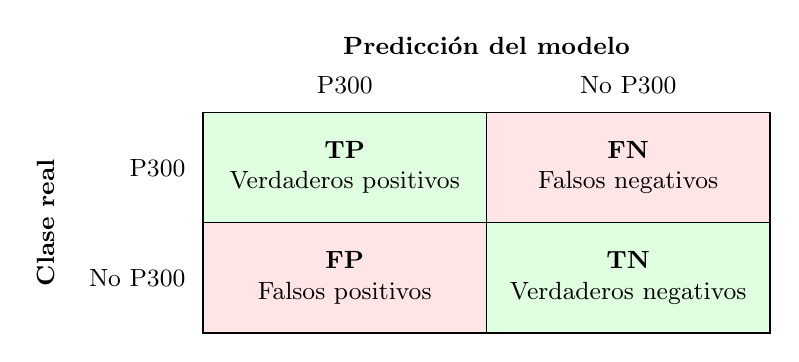
\begin{tikzpicture}[celda/.style={draw, minimum width=3.6cm, minimum height=1.4cm, align=center, font=\small}]
  \node[celda, fill=green!12] (tp) at (0,0) {\textbf{TP}\\Verdaderos positivos};
  \node[celda, fill=red!10] (fn) at (3.6,0) {\textbf{FN}\\Falsos negativos};
  \node[celda, fill=red!10] (fp) at (0,-1.4) {\textbf{FP}\\Falsos positivos};
  \node[celda, fill=green!12] (tn) at (3.6,-1.4) {\textbf{TN}\\Verdaderos negativos};
  \node[font=\small] at (0,1.05) {P300};
  \node[font=\small] at (3.6,1.05) {No P300};
  \node[font=\small\bfseries] at (1.8,1.55) {Predicción del modelo};
  \node[font=\small, anchor=east] at (-1.9,0) {P300};
  \node[font=\small, anchor=east] at (-1.9,-1.4) {No P300};
  \node[font=\small\bfseries, rotate=90] at (-3.8,-0.7) {Clase real};
\end{tikzpicture}
\caption{Matriz de confusión para la clasificación binaria de épocas. Elaboración propia.}
\label{fig:confusion}
\end{figure}

\subsection{Métricas de clasificación}

A partir de estos cuatro valores se calculan las métricas que se presentan en la
Tabla~\ref{tab:metricas}. La exactitud mide el porcentaje total de aciertos, pero como se discutió
en la Sección~\ref{sec:speller}, en un conjunto con una proporción de 1 a 5 entre clases puede
resultar engañosa, por lo que conviene complementarla con la sensibilidad, que indica qué
proporción de las épocas con P300 fueron detectadas, la precisión, que indica qué proporción de las
detecciones fueron correctas, y el F1-score, que es la media armónica de ambas
\cite{fawcett2006}. La exactitud balanceada, que promedia la sensibilidad y la especificidad, es
otra alternativa que no se ve afectada por el desbalance.

\begin{table}[htbp]
\centering
\caption{Métricas de evaluación para la clasificación binaria}
\label{tab:metricas}
\small
\begin{tabularx}{\textwidth}{L{2.8cm}YL{4.4cm}}
\toprule
\textbf{Métrica} & \textbf{Descripción} & \textbf{Fórmula} \\
\midrule
Exactitud (\textit{accuracy}) & Proporción de predicciones correctas sobre el total. & $\dfrac{TP+TN}{TP+TN+FP+FN}$ \\[10pt]
Precisión (\textit{precision}) & Proporción de épocas clasificadas como P300 que realmente lo son. & $\dfrac{TP}{TP+FP}$ \\[10pt]
Sensibilidad (\textit{recall}, TPR) & Proporción de épocas con P300 que fueron detectadas. & $\dfrac{TP}{TP+FN}$ \\[10pt]
Especificidad (TNR) & Proporción de épocas sin P300 clasificadas correctamente. & $\dfrac{TN}{TN+FP}$ \\[10pt]
Tasa de falsos positivos (FPR) & Proporción de épocas sin P300 clasificadas como positivas. & $\dfrac{FP}{FP+TN} = 1-\text{TNR}$ \\[10pt]
F1-score & Media armónica entre precisión y sensibilidad. & $2\cdot\dfrac{\text{Precisión}\cdot\text{Sensibilidad}}{\text{Precisión}+\text{Sensibilidad}}$ \\[10pt]
Exactitud balanceada & Promedio de la sensibilidad y la especificidad. & $\dfrac{\text{TPR}+\text{TNR}}{2}$ \\
\bottomrule
\end{tabularx}
\par\smallskip{\footnotesize Elaboración propia con información de \cite{fawcett2006}.}
\end{table}

\subsection{Curva ROC y área bajo la curva}

Los clasificadores de la P300 suelen producir un puntaje continuo, y la etiqueta final depende del
umbral que se elija: al disminuirlo se detectan más épocas con P300, pero también aumentan los
falsos positivos. La curva ROC (\textit{Receiver Operating Characteristic}) representa este
compromiso graficando la sensibilidad contra la tasa de falsos positivos para todos los umbrales
posibles, y el área bajo esta curva (AUC) resume el desempeño en un solo número que puede
interpretarse como la probabilidad de que el clasificador asigne un puntaje mayor a una época
positiva elegida al azar que a una negativa elegida al azar \cite{fawcett2006}. Un AUC de 0.5
corresponde a un clasificador aleatorio, cuyas distribuciones de puntajes para ambas clases se
encuentran superpuestas, mientras que un AUC de 1 indica una separación perfecta, como se ilustra
en la Figura~\ref{fig:roc}; esta es la métrica utilizada en los trabajos de Alvarado-González et al.
y de Contreras, en el que se considera aceptable a partir de 0.7 \cite{alvarado2021,contreras2021}.

\begin{figure}[htbp]
\centering

\includegraphics[width=\textwidth]{02-marco-referencial/roc_auc.pdf}
\caption{(a) Distribuciones de puntajes de un clasificador para ambas clases y un umbral de
decisión. (b) Curvas ROC para distintos grados de separación entre clases. Elaboración propia.}
\label{fig:roc}
\end{figure}

\subsection{Métricas a nivel de sistema}

Una alta AUC en la clasificación de épocas no garantiza por sí sola una comunicación eficiente,
pues la velocidad depende también del número de repeticiones necesarias para seleccionar cada
carácter. Por ello, en los sistemas de deletreo se reporta la exactitud por carácter en función
del número de repeticiones, los caracteres por minuto y la tasa de transferencia de información
(ITR), que de acuerdo con Wolpaw et al. se calcula en bits por selección como
\cite{wolpaw2000,wolpaw2002}
\begin{equation}
B = \log_2 N + P\log_2 P + (1-P)\log_2\!\left(\frac{1-P}{N-1}\right),
\label{eq:itr}
\end{equation}
donde $N$ es el número de opciones posibles, 36 en una matriz de $6\times6$, y $P$ es la exactitud
por carácter; al multiplicar $B$ por el número de selecciones por minuto se obtiene la ITR en bits
por minuto. La Figura~\ref{fig:itr} muestra que, para una misma exactitud, reducir el número de
repeticiones incrementa notablemente la ITR, aunque en la práctica disminuir las repeticiones
también reduce la exactitud, por lo que el número óptimo de repeticiones es aquel que maximiza el
producto de ambos efectos.

\begin{figure}[htbp]
\centering

\includegraphics[width=\textwidth]{02-marco-referencial/itr_repeticiones.pdf}
\caption{(a) Bits por selección en función de la exactitud para $N=36$ según la
Ecuación~\eqref{eq:itr}. (b) ITR teórica en función del número de repeticiones para tres niveles
de exactitud, considerando 175~ms por intensificación y 2.5~s entre caracteres. Elaboración
propia.}
\label{fig:itr}
\end{figure}

% ---------------------------------------------------------------------
% 2.12 Reducción de canales y repeticiones
% ---------------------------------------------------------------------
\section[REDUCCIÓN DE CANALES Y REPETICIONES]{Reducción de canales y repeticiones}

Como se señaló en la introducción, los sistemas P300 basados en EEG suelen alcanzar una alta
exactitud a costa de utilizar muchos electrodos y de repetir varias veces la estimulación de cada
fila y columna. Ambos factores afectan directamente la practicidad del sistema: un mayor número de
canales incrementa el costo del equipo y el tiempo necesario para colocar los electrodos, además de
dificultar su uso fuera del laboratorio, mientras que un mayor número de repeticiones reduce la
velocidad de comunicación y aumenta la fatiga del usuario \cite{krusienski2008,contreras2021}.

\subsection{Selección de canales}

La selección de canales busca identificar el subconjunto mínimo de electrodos que conserve la
información necesaria para detectar la P300. Krusienski et al. evaluaron distintos conjuntos de
electrodos y encontraron que un conjunto de ocho canales, Fz, Cz, Pz, P3, P4, PO7, PO8 y Oz, que
combina posiciones de la línea media con posiciones parieto-occipitales, ofrecía un desempeño
superior al de los tres canales de la línea media utilizados tradicionalmente \cite{krusienski2008}.
Por otra parte, Cecotti y Gräser aprovecharon los pesos aprendidos por la capa espacial de su CNN
para ordenar los electrodos según su contribución a la clasificación y eliminar los menos
relevantes \cite{cecotti2011}, estrategia que resulta natural en arquitecturas como EEGNet, cuya
convolución \textit{depthwise} aprende explícitamente un peso por electrodo \cite{lawhern2018}. En
el extremo opuesto, Contreras trabajó con solo cuatro electrodos de la línea media y obtuvo valores
de AUC aceptables en la evaluación intrasujeto \cite{contreras2021}.

\subsection{Reducción de repeticiones}

De acuerdo con la Ecuación~\eqref{eq:promediado}, cada repetición adicional mejora la relación
señal-ruido de la P300 en un factor proporcional a $\sqrt{N}$, pero también añade alrededor de
2.1~s al tiempo de cada selección con los parámetros de la base de datos utilizada. Una primera
estrategia para reducir las repeticiones consiste en mejorar la clasificación de ensayo único, es
decir, la capacidad del modelo de detectar la P300 en una sola época sin promediarla con otras,
objetivo que persiguen las arquitecturas convolucionales descritas en la Sección~\ref{sec:cnn}
\cite{cecotti2011,lawhern2018}. Una segunda estrategia es la parada dinámica, en la que el sistema
deja de presentar repeticiones en cuanto la confianza acumulada sobre algún carácter supera un
umbral, en lugar de usar siempre un número fijo; Speier et al. mostraron que combinar este tipo de
clasificación dinámica con información del lenguaje mejora tanto la exactitud como la tasa de
transferencia del P300 Speller \cite{speier2012}.

% ---------------------------------------------------------------------
% 2.13 Modelado del lenguaje y predicción de palabras
% ---------------------------------------------------------------------
\section[MODELADO DEL LENGUAJE Y PREDICCIÓN DE PALABRAS]{Modelado del lenguaje y predicción de
palabras}
\label{sec:lenguaje}

\subsection{Predicción de palabras en la comunicación asistida}

Aun con una detección perfecta de la P300, escribir carácter por carácter en un P300 Speller es un
proceso lento, pues cada selección requiere varios segundos. La predicción de palabras, ampliamente
utilizada en los sistemas de comunicación aumentativa, reduce el número de selecciones necesarias
al ofrecer al usuario una lista de palabras probables a partir de los caracteres que ya ha escrito,
de modo que puede completar una palabra con una sola selección adicional. Ryan et al. integraron
este mecanismo en un P300 Speller agregando a la matriz una región con las palabras sugeridas, y
encontraron que los participantes completaban las frases en menos tiempo que con el deletreador
convencional, aunque con una exactitud por selección ligeramente menor \cite{ryan2011}. El
beneficio de estos sistemas suele medirse mediante el ahorro de selecciones,
\begin{equation}
\text{AS} = \frac{S_{\text{sin}} - S_{\text{con}}}{S_{\text{sin}}}\times100\%,
\label{eq:ahorro}
\end{equation}
donde $S_{\text{sin}}$ y $S_{\text{con}}$ son el número de selecciones necesarias para escribir un
mismo texto sin y con predicción, respectivamente.

\subsection{Modelos de lenguaje probabilísticos}

Un modelo de lenguaje asigna una probabilidad a cada secuencia de palabras $w_1, \dots, w_m$, lo
que permite estimar cuál es la palabra, o el carácter, más probable dado lo que se ha escrito. Por
la regla de la cadena, esta probabilidad puede descomponerse como el producto de probabilidades
condicionales, y los modelos de $n$-gramas la aproximan suponiendo que cada palabra depende
únicamente de las $n-1$ anteriores, supuesto conocido como de Markov \cite{jurafsky2025}:
\begin{equation}
P(w_1,\dots,w_m) = \prod_{i=1}^{m} P(w_i \mid w_1,\dots,w_{i-1}) \approx \prod_{i=1}^{m} P(w_i \mid w_{i-n+1},\dots,w_{i-1}).
\label{eq:ngramas}
\end{equation}
Las probabilidades condicionales se estiman contando las frecuencias de aparición en un corpus de
texto, y dado que muchas secuencias válidas no aparecen en él, se aplican técnicas de suavizado que
reservan parte de la probabilidad para eventos no observados \cite{jurafsky2025}. La calidad de un
modelo de lenguaje se evalúa comúnmente mediante la perplejidad, $PP = P(w_1,\dots,w_m)^{-1/m}$,
que puede interpretarse como el número promedio de opciones entre las que el modelo duda en cada
paso, concepto que se relaciona directamente con la noción de entropía de la teoría de la
información de Shannon \cite{shannon1948,jurafsky2025}.

\subsection{Modelos de lenguaje neuronales}

Los modelos de $n$-gramas están limitados a un contexto corto y fijo, por lo que fueron
reemplazados progresivamente por modelos neuronales. Las redes recurrentes, y en particular las
LSTM, permitieron condicionar la predicción en un contexto de longitud variable
\cite{hochreiter1997,jurafsky2025}, y posteriormente la arquitectura Transformer, basada
exclusivamente en mecanismos de atención, eliminó la recurrencia y permitió entrenar modelos
mucho más grandes de forma paralela \cite{vaswani2017}. Sobre esta arquitectura se construyen los
modelos de lenguaje de gran escala (LLM), entrenados con enormes cantidades de texto, que son
capaces de realizar tareas nuevas a partir de unas cuantas instrucciones o ejemplos
\cite{brown2020}.

\subsection{Integración del lenguaje en el P300 Speller}

La información del lenguaje puede incorporarse al P300 Speller de dos maneras: como sugerencias
explícitas que el usuario selecciona, o como una probabilidad previa que se combina con los
puntajes del clasificador para decidir el carácter. Speier et al. siguieron la segunda vía,
integrando un modelo de lenguaje en el proceso de clasificación dinámica, y reportaron mejoras
tanto en la exactitud como en la tasa de transferencia de información \cite{speier2012}. Más
recientemente, Hong et al. propusieron ChatBCI, un P300 Speller que utiliza un LLM para predecir
palabras según el contexto de la frase, logrando una reducción del tiempo promedio de escritura de
62.14\% \cite{hong2026}. La Tabla~\ref{tab:lenguaje} compara estos enfoques.

\begin{table}[htbp]
\centering
\caption{Trabajos que integran modelos de lenguaje en el P300 Speller}
\label{tab:lenguaje}
\small
\begin{tabularx}{\textwidth}{L{3.0cm}L{3.2cm}YY}
\toprule
\textbf{Trabajo} & \textbf{Modelo de lenguaje} & \textbf{Forma de integración} & \textbf{Resultado} \\
\midrule
Ryan et al., 2011 \cite{ryan2011} & Predicción de palabras por diccionario & Región adicional con palabras sugeridas en la interfaz. & Menor tiempo para completar frases, con exactitud ligeramente menor. \\
Speier et al., 2012 \cite{speier2012} & Modelo probabilístico de lenguaje natural & Probabilidad previa combinada con la clasificación dinámica. & Mejor exactitud y tasa de transferencia. \\
Hong et al., 2026 \cite{hong2026} & LLM & Predicción contextual de palabras. & Reducción del tiempo promedio de 62.14\%. \\
\bottomrule
\end{tabularx}
\par\smallskip{\footnotesize Elaboración propia.}
\end{table}

% ---------------------------------------------------------------------
% 2.14 Estado del arte
% ---------------------------------------------------------------------
\section[ESTADO DEL ARTE]{Estado del arte}

\subsection{Sistemas P300 Speller y competencias BCI}

A partir del deletreador de Farwell y Donchin \cite{farwell1988}, la investigación sobre el P300
Speller se centró durante varios años en mejorar la clasificación de las épocas con métodos
lineales. Las competencias internacionales de BCI jugaron un papel central en este proceso, pues
pusieron a disposición de la comunidad bases de datos comunes; en la tercera de ellas, el conjunto
de SVM lineales propuesto por Rakotomamonjy y Guigue obtuvo el primer lugar al identificar
correctamente el 96.5\% de los caracteres de prueba con 15 repeticiones \cite{rakotomamonjy2008}.
En paralelo, Krusienski et al. mostraron que el SWLDA y el discriminante de Fisher eran los
clasificadores más robustos entre los evaluados \cite{krusienski2006}, y posteriormente que una
adecuada selección de ocho electrodos permitía mejorar el desempeño respecto al uso exclusivo de la
línea media \cite{krusienski2008}.

\subsection{Sistemas de comunicación con usuarios con discapacidad}

La validación con usuarios reales ha sido otra línea importante de investigación. Sellers y
Donchin realizaron las primeras pruebas de un P300 Speller con pacientes con ELA
\cite{sellers2006}, y Hoffmann et al. propusieron un sistema de seis opciones evaluado con personas
con distintas discapacidades motoras, cuyos registros constituyen hoy una de las bases de datos
públicas más utilizadas \cite{hoffmann2008}. En el ámbito latinoamericano, el estudio ``Interfaz
cerebro-computador basada en P300 para la comunicación alternativa'' \cite{garciacossio2011}
implementó un sistema funcional de deletreo utilizando una matriz de estimulación visual con dos
adolescentes en situación de discapacidad motora, reportando porcentajes de acierto promedio de 95\%
y 85\% para cada usuario en la prueba de libre deletreo. Por su parte, el trabajo de Brunner et
al. \cite{brunner2011} demostró la operación de un sistema P300 Speller utilizando señales de
electrocorticografía, alcanzando tasas sostenidas superiores a 17 caracteres por minuto; no
obstante, el uso de técnicas invasivas limita su aplicación en contextos clínicos generales, donde
el EEG continúa siendo la alternativa más accesible.

\subsection{Aprendizaje profundo para la detección de la P300}

Con la introducción de las redes convolucionales, Cecotti y Gräser mostraron que era posible
aprender directamente los filtros espaciales y temporales a partir de la señal, obteniendo en la
competencia BCI III resultados comparables a los del ganador \cite{cecotti2011}. A partir de
entonces se propusieron arquitecturas como BN3 \cite{liu2018}, OCLNN \cite{shan2018} y EEGNet
\cite{lawhern2018}, y la comparación de Alvarado-González et al. mostró que redes muy compactas
como SepConv1D, con apenas cuatro filtros en su única capa convolucional, pueden alcanzar un AUC
similar a la de redes mucho más grandes \cite{alvarado2021}.

En el ámbito nacional, la tesis de maestría titulada ``Sistema clasificador de señales EEG para
el control de una neuroprótesis por medio de un dispositivo móvil'' \cite{contreras2021},
desarrollada en la Escuela Superior de Cómputo del Instituto Politécnico Nacional, implementó un
sistema basado en la arquitectura SepConv1D para la detección del componente P300 con solo cuatro
electrodos secos, reportando valores promedio de AUC cercanos a 0.82 en evaluaciones intrasujeto y
de 0.70 en escenarios intersujeto sin calibración individual al considerar filas y columnas. Este
trabajo demostró la viabilidad técnica de integrar procesamiento EEG, extracción automática de
características y modelos de aprendizaje profundo en un sistema funcional; sin embargo, su
aplicación estuvo orientada al control de una neuroprótesis y no específicamente a la
implementación de un sistema de comunicación mediante deletreo. En la misma escuela, Santos,
Romero y Fernández desarrollaron una aplicación para manipular un brazo robótico virtual mediante
potenciales P300 con matrices de $5\times5$ de iconos y de letras, clasificadas con el
discriminante lineal de Fisher \cite{santos2017}, y Anguiano y Ramírez utilizaron señales de EEG
y redes neuronales artificiales para detectar estrés en estudiantes \cite{anguiano2019}.

\subsection{Modelos de lenguaje en el P300 Speller}

La incorporación de información lingüística es la línea más reciente para acelerar la escritura.
Ryan et al. \cite{ryan2011} y Speier et al. \cite{speier2012} mostraron que la predicción de
palabras y los modelos de lenguaje reducen el tiempo de escritura o mejoran la tasa de
transferencia, y más recientemente la investigación ``ChatBCI'' \cite{hong2026} incorporó modelos
de lenguaje de gran escala para mejorar las selecciones dentro de un sistema P300 Speller, logrando
una reducción del tiempo promedio de escritura de 62.14\%.

\subsection{Resumen comparativo}

De los trabajos revisados se identifican dos limitaciones persistentes en los sistemas P300
basados en EEG: la necesidad de múltiples canales para mantener niveles altos de precisión y la
dependencia de múltiples repeticiones de estímulos para asegurar una detección confiable. La
Tabla~\ref{tab:estado-arte} resume los enfoques descritos, contrastando el número de canales
empleados, el clasificador, el uso de un modelo de lenguaje y el desempeño reportado por cada
trabajo frente a la propuesta del presente Trabajo Terminal.

\begin{table}[htbp]
\centering
\caption{Resumen comparativo del estado del arte}
\label{tab:estado-arte}
\footnotesize
\begin{tabularx}{\textwidth}{L{3.1cm}L{1.8cm}L{2.4cm}L{2.1cm}Y}
\toprule
\textbf{Trabajo} & \textbf{Señal / canales} & \textbf{Clasificador} & \textbf{Modelo de lenguaje} & \textbf{Desempeño} \\
\midrule
Farwell y Donchin, 1988 \cite{farwell1988} & EEG / 1 (Pz) & SWDA, pico, área y covarianza & No & Exactitud $\approx$ 95\%; 2.3 caracteres/min \\
Sellers y Donchin, 2006 \cite{sellers2006} & EEG & -- & No & Primeras pruebas con pacientes con ELA \\
Rakotomamonjy y Guigue, 2008 \cite{rakotomamonjy2008} & EEG / 64 & Conjunto de SVM & No & 96.5\% de caracteres con 15 repeticiones \\
Krusienski et al., 2008 \cite{krusienski2008} & EEG / 8 & SWLDA & No & Conjunto de 8 canales superior a la línea media \\
Cecotti y Gräser, 2011 \cite{cecotti2011} & EEG / 64 & CNN & No & $\approx$ 95\% de caracteres con 15 repeticiones \\
García Cossio et al., 2011 \cite{garciacossio2011} & EEG / 6 & -- & No & Acierto de 95\% y 85\% en libre deletreo \\
Brunner et al., 2011 \cite{brunner2011} & ECoG / 96 subdurales & SWLDA & No & 17 caracteres/min \\
Ryan et al., 2011 \cite{ryan2011} & EEG & -- & Diccionario & Menor tiempo por frase \\
Speier et al., 2012 \cite{speier2012} & EEG & Clasificación dinámica & Probabilístico & Mayor exactitud y tasa de transferencia \\
Santos et al., 2017 (ESCOM) \cite{santos2017} & EEG & LDA de Fisher & No & Precisión de 90.01\% (20 sujetos) \\
Alvarado-González et al., 2021 \cite{alvarado2021} & EEG / varios & SepConv1D y otras 11 redes & No & AUC intra $\approx$ 0.84; inter $\approx$ 0.78 \\
Contreras, 2021 (IPN) \cite{contreras2021} & EEG / 4 & SepConv1D & No & AUC $\approx$ 0.82 (intrasujeto), $\approx$ 0.70 (intersujeto) \\
ChatBCI, Hong et al., 2026 \cite{hong2026} & EEG / 32 & -- & LLM & Reducción de tiempo promedio de 62.14\% \\
\midrule
\textbf{Propuesta TT} & EEG / 4 & Aprendizaje profundo (CNN) & Predicción de palabras & -- \\
\bottomrule
\end{tabularx}
\par\smallskip{\footnotesize Elaboración propia.}
\end{table}

